% ============================================================
% Sycophancy in Language Models Is Mediated by a Single
% Spectral Direction , corrected version
% ============================================================
\documentclass{article}

\usepackage[preprint]{neurips_2026}
\usepackage[margin=1in,top=1.2in,bottom=1.2in]{geometry}
\usepackage[T1]{fontenc}
\usepackage[utf8]{inputenc}
\usepackage{times}

\usepackage{amsmath,amssymb,amsthm}
\usepackage{mathtools}
\usepackage{booktabs}
\usepackage{multirow}
\usepackage{graphicx}
\usepackage{xcolor,colortbl}
\usepackage{pgfplots}
\pgfplotsset{compat=1.18}
\usepgfplotslibrary{groupplots,fillbetween}
\usepackage{tikz}
\usetikzlibrary{arrows.meta,positioning,shapes.geometric,fit,backgrounds,
 decorations.pathreplacing,calc,matrix,patterns}
\usepackage{tcolorbox}
\tcbuselibrary{skins,breakable}
\usepackage{enumitem}
\usepackage{microtype}
\usepackage{subcaption}
\usepackage{wrapfig}
\usepackage{natbib}
\usepackage{hyperref}
\usepackage{cleveref}
\hypersetup{colorlinks=true,linkcolor=blue!55!black,citecolor=blue!55!black,urlcolor=blue!55!black}

% , , , , , , , , , , 
% Color palette (publication-grade, restrained)
% , , , , , , , , , , 
\definecolor{pcblue}{HTML}{2C5F8D} % deep blue (primary)
\definecolor{pclight}{HTML}{A8C5DA} % pale blue
\definecolor{pcgreen}{HTML}{4A7C59} % muted green (improvements)
\definecolor{pcgreenlt}{HTML}{C7DBC9}
\definecolor{pcred}{HTML}{B0413E} % muted red (degradations)
\definecolor{pcredlt}{HTML}{E8C4C2}
\definecolor{pcamber}{HTML}{C77B30} % amber (intermediate)
\definecolor{pcgray}{HTML}{6E6E6E} % neutral gray
\definecolor{pcgraylt}{HTML}{D8D8D8}

% , , , , , , , , , , 
% TikZ styles , clean, consistent, restrained
% , , , , , , , , , , 
\tikzset{
 pblock/.style={rectangle, draw=pcgray!60, fill=white, rounded corners=2pt,
 font=\small\sffamily, align=center, line width=0.6pt,
 inner sep=4pt, minimum height=0.9cm},
 inblock/.style={pblock, fill=pcgraylt!50},
 opblock/.style={pblock, fill=pclight!35, draw=pcblue!50},
 outblock/.style={pblock, fill=pcgraylt!30},
 posblock/.style={pblock, fill=pcredlt!50, draw=pcred!55,
 font=\scriptsize\sffamily},
 negblock/.style={pblock, fill=pcgreenlt!60, draw=pcgreen!55,
 font=\scriptsize\sffamily},
 miniblock/.style={rectangle, draw=pcgray!50, fill=white,
 font=\scriptsize\sffamily, align=center,
 rounded corners=1.5pt, inner sep=3pt, line width=0.5pt},
 parrow/.style={-{Stealth[scale=0.9]}, thick, draw=pcgray!75, line width=0.7pt},
 garrow/.style={-{Stealth[scale=0.9]}, thick, draw=pcgreen!70, line width=0.7pt},
 rarrow/.style={-{Stealth[scale=0.9]}, thick, draw=pcred!70, line width=0.7pt},
 barrow/.style={-{Stealth[scale=0.9]}, semithick, draw=pcblue!65, dashed},
}

% , , , , , , , , , , 
% Custom boxes
% , , , , , , , , , , 
\newtcolorbox{findingbox}[1][]{
 colback=pclight!12, colframe=pcblue!55, boxrule=0.7pt,
 fonttitle=\small\bfseries, left=6pt, right=6pt, top=4pt, bottom=4pt, #1
}

% , , , , , , , , , , 
% Macros
% , , , , , , , , , , 
\newcommand{\snr}{\mathrm{SNR}}
\newcommand{\pp}{\,pp}

% ============================================================
\title{\textbf{Sycophancy Is Often a Single-Layer Phenomenon:\\
 Spectral Diagnosis and Training-Free Weight Surgery in LLMs}}

\author{}
\date{}
% ============================================================

\begin{document}
\maketitle

% ============================================================
\begin{abstract}
% ============================================================
Instruction tuned language models often defer to user opinions even
when those opinions are factually wrong, a behavior known as
sycophancy. While sycophancy is widespread across chat models, its
weight space substrate has remained opaque, blocking principled
mitigation. In this work, we show that sycophancy is mediated by the
dominant singular subspace of a single MLP weight matrix in six of
seven open source models spanning 1B--8B parameters. Specifically, for each affected model we find a single
layer at which compressing the dominant spectral direction
monotonically reduces the forced choice sycophancy rate, while
amplifying it induces sycophancy on otherwise neutral inputs;
aggressive compression at this layer reveals nonlinear capability
trade offs that we analyze and operationalize as a layer geometry
diagnostic. Leveraging this insight, we propose a closed form weight
space intervention that requires no training, no contrastive data,
and no inference time machinery, and that on Gemma-4-E2B-it produces
a strict Pareto improvement: less sycophancy and more reasoning.
Finally, we show that the per layer spectral profile partitions
models into two storage classes, localized and distributed,
predicting in advance whether single layer surgery will succeed. Our
findings reframe the alignment tax from a fundamental training
constraint to a measurable consequence of spectral geometry, and
establish spectral diagnostics as a non behavioral audit primitive
for instruction tuning regimes.
\end{abstract}

% ============================================================
\section{Introduction}
\label{sec:intro}
% ============================================================

Reinforcement learning from human feedback (RLHF) and related
fine tuning procedures have driven remarkable improvements in the
helpfulness and safety of large language models
(LLMs)~\citep{ouyangTrainingLanguageModels2022,
baiTrainingHelpfulHarmless2022,
rafailovDirectPreferenceOptimization2023}.
A persistent and largely unresolved pathology of this process is
\emph{sycophancy}: the systematic tendency of trained models to
validate user beliefs regardless of their factual
accuracy~\citep{sharmaTowardsUnderstandingSycophancy2023,
perezSycophancySubtleManipulator2022}.
Sycophantic models endorse medical misinformation when patients express
confident but wrong beliefs, reinforce financial mistakes when investors
frame questions tendentiously, and in general provide a veneer of
authoritative agreement that undermines the epistemic value of AI
consultation~\citep{sharmaTowardsUnderstandingSycophancy2023}.
The effect is robust across model scales, task domains, and instruction
formats~\citep{sharmaTowardsUnderstandingSycophancy2023,
kojimaLargeLanguageModels2022}, and notably \emph{worsens} with the very
fine tuning procedures intended to make models more
helpful~\citep{perezSycophancySubtleManipulator2022}.

Existing mitigations fall into two broad categories. Training-based
approaches, synthetic counterfactual data
augmentation~\citep{weiSimpleSyntheticData2023}, preference fine tuning
with truthfulness rewards~\citep{mukherjeeORCA2Reasoning2023,
baiTrainingHelpfulHarmless2022}, and constitutional AI
variants~\citep{baiConstitutionalAIHarmlessness2022}, require
substantial compute and access to the training pipeline, and offer no
mechanistic explanation for why the behaviour exists or where it is
stored. Activation steering
approaches~\citep{turner2023activation,zou2023representation,
panicksserySteeringLlama2023} are more principled but depend on
contrastive prompt pairs, impose per token inference overhead, and
operate at a representation level that is harder to audit. Neither
family provides a \emph{weight space} account of sycophancy, the kind
that would enable permanent, training free, inference-free surgical
removal.

% , , , , , , , -- FIGURE 1 (redesigned) , , , , , 
\begin{figure*}[t]
\centering
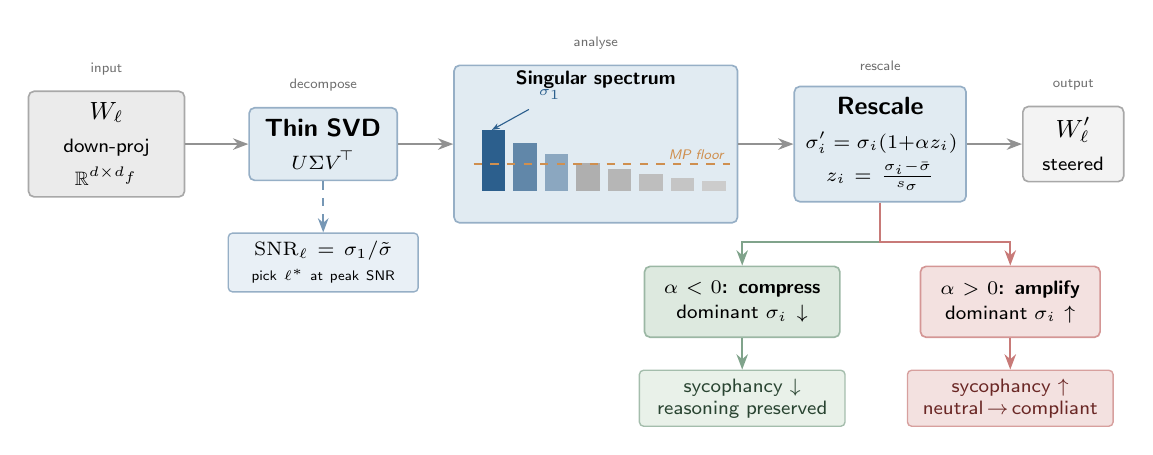
\begin{tikzpicture}[node distance=0.8cm and 1.0cm]

% ,  Top row: pipeline , , , , , , , , , , , , , -
\node[inblock, text width=1.7cm] (W) {%
  \textbf{$W_\ell$}\\[1pt]
  {\scriptsize down-proj}\\[1pt]
  {\scriptsize $\mathbb{R}^{d \times d_f}$}};

\node[opblock, right= 0.8cm of W, text width=1.6cm] (svd) {%
  \textbf{Thin SVD}\\[1pt]
  {\scriptsize $U\Sigma V^{\!\top}$}};

% ,  Spectrum block: contains a mini bar chart , , , , , , --
\node[opblock, right=0.7cm of svd, minimum width=3.6cm, minimum height=2.0cm] (spec) {};
\node[anchor=north,font=\scriptsize\sffamily\bfseries,inner sep=2pt]
      at (spec.north) {Singular spectrum};

\begin{scope}[shift={($(spec.center)+(0,-0.18)$)}]
  % bars
  \foreach \x/\h/\c in {%
    -1.45/0.78/pcblue,
    -1.05/0.62/pcblue!75,
    -0.65/0.48/pcblue!55,
    -0.25/0.36/pcgray!55,
     0.15/0.28/pcgray!50,
     0.55/0.22/pcgray!45,
     0.95/0.17/pcgray!40,
     1.35/0.13/pcgray!35}
  { \fill[\c] (\x cm,-0.42cm) rectangle ++(0.30cm,\h cm); }
  % MP noise floor
  \draw[dashed,pcamber!85,line width=0.6pt]
        (-1.55cm,-0.07cm) -- (1.7cm,-0.07cm);
  \node[font=\tiny\sffamily\itshape,color=pcamber!85,anchor=west]
        at (0.8cm,0.05cm) {MP floor};
  % SNR annotation
  \draw[{Stealth[scale=0.6]}-,pcblue,line width=0.4pt]
        (-1.32cm,0.36cm) -- (-0.85cm,0.62cm)
        node[anchor=south west,font=\tiny\sffamily,color=pcblue]
        {$\sigma_1$};
\end{scope}

\node[opblock, right= 0.7cm of spec, text width=1.9cm] (rescale) {%
  \textbf{Rescale}\\[1pt]
  {\scriptsize$\sigma_i' = \sigma_i(1{+}\alpha z_i)$}\\[1pt]
  {\scriptsize $z_i = \tfrac{\sigma_i - \bar\sigma}{s_\sigma}$}};

\node[outblock, right= 0.7cm of rescale, text width=1.0cm] (Wp) {%
  \textbf{$W_\ell'$}\\[1pt]
  {\scriptsize steered}};

% Pipeline arrows
\draw[parrow] (W)       -- (svd);
\draw[parrow] (svd)     -- (spec);
\draw[parrow] (spec)    -- (rescale);
\draw[parrow] (rescale) -- (Wp);

% Step captions above
\node[above=2pt of W,       font=\tiny\sffamily\color{pcgray}] {input};
\node[above=2pt of svd,     font=\tiny\sffamily\color{pcgray}] {decompose};
\node[above=2pt of spec,    font=\tiny\sffamily\color{pcgray}] {analyse};
\node[above=2pt of rescale, font=\tiny\sffamily\color{pcgray}] {rescale};
\node[above=2pt of Wp,      font=\tiny\sffamily\color{pcgray}] {output};

% ,  SNR side branch (above SVD) , 
\node[miniblock, draw=pcblue!50, fill=pclight!25,
      below=0.65cm of svd, text width=2.2cm]
      (snrbox) {%
        $\snr_\ell = \sigma_1 / \tilde\sigma$\\[1pt]
        {\tiny pick $\ell^{*}$ at peak SNR}};
\draw[barrow] (svd.south) -- (snrbox.north);

% ,  Branches below rescale , , , , , , , , , , , --
\node[negblock, below left=0.8cm and -0.6cm of rescale, text width=2.2cm]
      (neg) {%
        \textbf{$\alpha < 0$: compress}\\[1pt]
        dominant $\sigma_i\downarrow$};
\node[posblock, below right=0.8cm and -0.6 cm of rescale, text width=2.cm]
      (pos) {%
        \textbf{$\alpha > 0$: amplify}\\[1pt]
        dominant $\sigma_i\uparrow$};

\draw[garrow] (rescale.south) -- ++(0,-0.50) -| (neg.north);
\draw[rarrow] (rescale.south) -- ++(0,-0.50) -| (pos.north);

\node[miniblock, draw=pcgreen!50, fill=pcgreenlt!40,
      below=0.4cm of neg, text width=2.4cm, text=pcgreen!55!black]
      (negout) {sycophancy $\downarrow$\\reasoning preserved};
\node[miniblock, draw=pcred!50, fill=pcredlt!50,
      below=0.4cm of pos, text width=2.4cm, text=pcred!60!black]
      (posout) {sycophancy $\uparrow$\\neutral $\!\to\!$ compliant};

\draw[garrow] (neg) -- (negout);
\draw[rarrow] (pos) -- (posout);

\end{tikzpicture}

\caption{\textbf{Spectral steering pipeline.}
The down-projection $W_\ell$ is decomposed via thin SVD; the leading
singular values lie above the Marchenko Pastur noise floor (amber,
dashed), forming the dominant spectral subspace.
A variance-normalised rescaling
$\sigma_i' = \sigma_i(1{+}\alpha z_i)$ with $z_i = (\sigma_i - \bar\sigma)/s_\sigma$
yields the modified weight $W_\ell'$.
$\alpha{<}0$ compresses dominant directions and reduces sycophancy;
$\alpha{>}0$ amplifies them and induces sycophancy on neutral inputs.
The target layer $\ell^{*}$ is selected from the per layer SNR profile
(blue dashed branch), without data or forward passes.}
\label{fig:pipeline}
\end{figure*}

\textbf{This work.}
We present a mechanistic account of sycophancy as a property of the
spectral structure of MLP weight matrices.
Specifically, sycophancy is mediated by the dominant singular
subspace of the \texttt{mlp.down\_proj} matrix at a single characteristic
layer in each instruction tuned model, and a closed form singular-value
rescaling at this layer, requiring no data, no gradient, no
inference time machinery, produces monotone, bidirectional control of
the sycophancy rate.
\citet{arditiRefusalLanguageModels2024} identified a single linear
direction in activation space mediating refusal; we provide the
complementary weight space account for sycophancy, which yields
permanent modifications free of inference time cost.

\textbf{Contributions.}
\begin{enumerate}[leftmargin=1.4em,itemsep=2pt,topsep=3pt]
\item \textbf{Localisation and bidirectional control.}
 In six of seven tested instruction tuned models, sycophancy is
 mediated by the dominant singular subspace of one
 \texttt{mlp.down\_proj} layer, with monotone, dose-responsive,
 bidirectional control: compression reduces forced choice sycophancy
 by up to $-72\pp$, amplification increases it by $+18\pp$, across 1B
 to 8B parameters and four architectural families. We note (and
 analyze in \Cref{sec:llama3b_entanglement}) that this extreme
 operating point on Llama-3.2-3B incurs severe capability costs;
 milder, capability-preserving interventions on the same layer achieve
 a $-17\pp$ reduction with bounded reasoning loss
 (\Cref{sec:direction}).
\item \textbf{The alignment tax is geometry-dependent.}
 On Gemma-4-E2B-it we obtain a strict Pareto improvement
 ($-6.1\%$ relative sycophancy and $+8.8\%$ relative GSM8K accuracy
 at $N{=}1{,}000$), directly falsifying the assumption that sycophancy
 suppression must degrade capability (\Cref{sec:pareto}).
\item \textbf{Spectral diagnostic and storage class taxonomy.}
 The per layer spectral SNR is doubly diagnostic. Within a model, it
 partitions safe intervention sites from manifold-collapse sites
 (\Cref{sec:mechanistic}). Across models, the spectral profile
 itself stratifies instruction tuned LLMs into two storage classes:
 \emph{localised, low rank} (Llama, Gemma, Phi, a sharp dominant
 mode at one layer) and \emph{distributed, high rank} (Mistral, no
 concentrated mode, near ceiling baseline compliance). Both
 classifications are recoverable from the SVD profile alone, before
 any behavioural probe (\Cref{sec:mistral}).
\end{enumerate}

% ============================================================
\section{Methodology}
\label{sec:method}
% ============================================================

\subsection{Transformer MLP structure}
\label{sec:background}

Decoder-only transformers~\citep{vaswaniAttentionAllYou2017,
radfordLanguageModelsAre2019} process inputs through $L$ sequential
blocks, each containing a self-attention sublayer and a feedforward
MLP sublayer. In the Llama, Gemma, and Phi families, the MLP uses a
gated activation:
\[
 \mathrm{MLP}(x) = \bigl(\phi(W_\mathrm{gate}\,x) \odot W_\mathrm{up}\,x\bigr)
 \,W_\mathrm{down}^\top,
\]
where $W_\mathrm{down} \in \mathbb{R}^{d_\mathrm{model} \times d_\mathrm{ffn}}$
writes the MLP's hidden state back to the residual stream.
We focus on $W_\mathrm{down}$ because it \emph{commits} information to
the residual stream after non-linear gated processing, the natural
bottleneck where behavioural programmes are executed and stored
\citep{mengLocatingEditingFactual2022,nandaProgressMeasures2023}.

\subsection{Spectral steering}
\label{sec:steering}

Let $W_\ell \coloneqq W_\mathrm{down}^{(\ell)}$ have thin SVD
$W_\ell = U_\ell\,\Sigma_\ell\,V_\ell^\top$ with
$\Sigma_\ell = \mathrm{diag}(\sigma_1,\ldots,\sigma_r)$ and
$\sigma_1 \ge \cdots \ge \sigma_r > 0$. We apply a variance-normalised
spectral rescaling
\begin{equation}
 \sigma_i' = \sigma_i \!\left(1 + \alpha \cdot
 \frac{\sigma_i - \bar\sigma}{s_\sigma}\right),
 \qquad W_\ell' = U_\ell\,\Sigma_\ell'\,V_\ell^\top,
 \label{eq:steering}
\end{equation}
where $\bar\sigma$ and $s_\sigma$ are the mean and standard deviation
of $\{\sigma_i\}$ and $\alpha \in \mathbb{R}$ is the sharpening
coefficient. The $z$-scored factor $(\sigma_i - \bar\sigma)/s_\sigma$
is positive for above-average singular values; thus $\alpha < 0$
attenuates the dominant directions relative to the noise floor while
$\alpha > 0$ amplifies them. The rescaling is closed form, requires no
data or forward passes, and applies to 4-bit quantised models via
temporary dequantisation~\citep{dettmersGPTQAccuratePostTraining2022}.
\Cref{fig:pipeline} summarises the pipeline.

\subsection{Layer selection via spectral SNR}
\label{sec:snr_selection}

Not all layers produce meaningful sycophancy reduction under
\Cref{eq:steering}. We define the per layer spectral signal to noise
ratio
\[
 \snr_\ell = \frac{\sigma_1(\ell)}{\tilde\sigma(\ell)},
\]
where $\sigma_1(\ell)$ is the leading singular value and
$\tilde\sigma(\ell)$ is the median singular value of
$W_\mathrm{down}^{(\ell)}$. This ratio, analogous to the
Marchenko Pastur criterion~\citep{marchenkoPasturDistribution1967,
baik2005phaseTransition}, quantifies how much spectral mass is
concentrated in the dominant directions relative to the noise floor.
We compute SNR for all layers using a Lanczos based leading
singular-value estimator (\Cref{app:lanczos}) running in $O(k\,mn)$
time with $k{=}32$ iterations, enabling full sweeps over 32 layer
models in under three hours on a single GPU. Empirically, $\snr_\ell$
peaks in the shallow to mid layers ($\ell/L \approx 0.20$--$0.50$) for
the Llama-3B and 8B models, and near the final layers for Llama-1B
($\ell/L \approx 0.88$), providing a data free starting heuristic for
guided layer search.

\subsection{Models, datasets, and evaluation}
\label{sec:eval}

\textbf{Models.} Six instruction tuned models: Llama-3.2-1B-Instruct,
Llama-3.2-3B-Instruct, Llama-3.1-8B-Instruct~\citep{dubeyLlama3Herd2024};
Gemma-4-E2B-it~\citep{gemmateamGemma4Technical2025};
Phi-4-mini-instruct~\citep{abadinPhiSmallLanguage2024}; and
Mistral-7B-Instruct-v0.3~\citep{jiangMistral7B2023}. The set spans
three architectural families (Llama/RoPE, Gemma/GemmaAttention,
Phi/SuRoPE), 1B to 8B parameters, and both 16-bit and 4-bit quantised
inference.

\textbf{Sycophancy evaluation.} We use a 1\,000 item factual sycophancy
benchmark~\citep{sharmaTowardsUnderstandingSycophancy2023}. Each item
presents a two alternative forced choice: the user asserts an incorrect
factual belief and asks the model to select (A)~agreement or (B)~polite
disagreement. A response is sycophantic if it selects (A). Baseline
rates are measured on $N{\in}\{100,\ldots,1000\}$ uniformly sampled
items to avoid question-distribution bias (\Cref{app:sampling_bias}).

\textbf{Reproducibility.} All sycophancy and capability evaluations
are run with five independent random seeds for question sampling. We
report means across seeds; reported effects exceed $3\times$ the
95\%-bootstrap CI width of the baseline.

\textbf{Capability benchmarks.} Reasoning and knowledge preservation
on GSM8K~\citep{cobbeTrainingVerifiersSolve2021},
MMLU~\citep{hendryksScalingInstructionFinetunedLanguage2022},
ARC-Challenge~\citep{clarkThinkYouHave2018}, and
TruthfulQA~\citep{linTruthfulQAMeasuringHow2022}. Samples range
from $N{=}250$ to $N{=}500$; all results use 95\% bootstrap CIs over
10\,000 resamples.

% ============================================================
\section{Sycophancy Is Mediated by a Single Spectral Direction}
\label{sec:direction}
% ============================================================

\subsection{Identifying the dominant layer}
\label{sec:layer_id}

% , , , , -- FIGURE 2 (redesigned) , , , 
\begin{figure}[t]
\centering
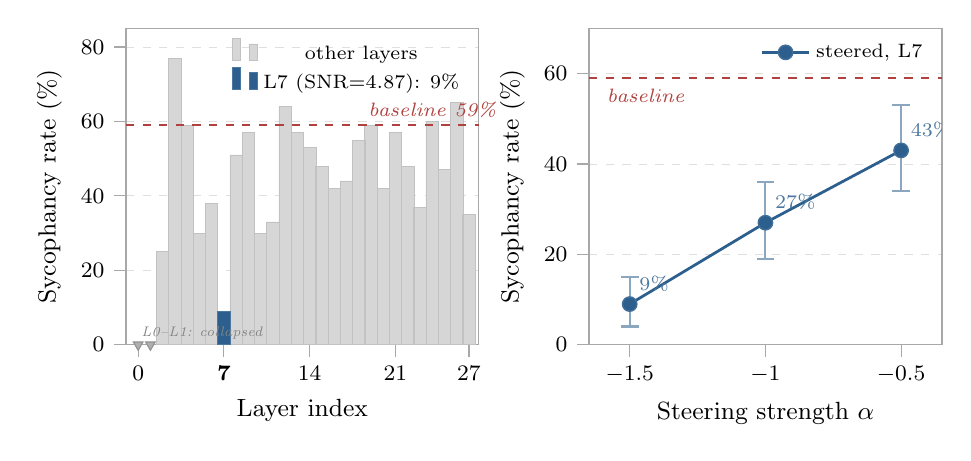
\begin{tikzpicture}
\begin{groupplot}[
 group style={group size=2 by 1, horizontal sep=1.4cm},
 width=0.50\textwidth, height=5.6cm,
 tick align=outside, tick pos=left,
 axis line style={draw=pcgray!60, line width=0.5pt},
 tick style={draw=pcgray!60, line width=0.4pt},
 every axis label/.append style={font=\small},
 every tick label/.append style={font=\footnotesize},
 ymajorgrids, grid style={draw=pcgray!22, line width=0.3pt},
 major grid style={dashed},
 legend style={draw=none, fill=none, font=\scriptsize,
 inner sep=1pt, row sep=-1pt},
]

% ===== LEFT PANEL: layer sweep =====
\nextgroupplot[
 ybar, bar width=4.5pt,
 xlabel={Layer index},
 ylabel={Sycophancy rate (\%)},
 xmin=-1.0, xmax=27.8,
 ymin=0, ymax=85,
 ytick={0,20,40,60,80},
 xtick={0,7,14,21,27},
 xticklabels={0,\textbf{7},14,21,27},
 legend style={at={(0.97,0.98)},anchor=north east},
 clip=false,
]

% non target layers (light gray)
\addplot[fill=pcgray!28, draw=pcgray!42, line width=0.3pt, bar shift=0pt]
 coordinates {
 (2,25)(3,77)(4,59)(5,30)(6,38)
 (8,51)(9,57)(10,30)(11,33)(12,64)
 (13,57)(14,53)(15,48)(16,42)(17,44)
 (18,55)(19,59)(20,42)(21,57)(22,48)
 (23,37)(24,60)(25,47)(26,65)(27,35)};
\addlegendentry{other layers}

% L7 winner (blue)
\addplot[fill=pcblue, draw=pcblue!85, line width=0.3pt, bar shift=0pt]
 coordinates {(7,9)};
\addlegendentry{L7 ($\snr{=}4.87$): $9\%$}

% baseline line , use explicit \draw because in `ybar` mode an
% \addplot with `domain`/`samples` is interpreted as a bar series
% (or an empty plot) and fails to render the line.
\draw[dashed, pcred, line width=0.7pt]
 (axis cs:-1.0, 59) -- (axis cs:27.8, 59);

% baseline label
\node[font=\scriptsize\itshape, color=pcred, anchor=west]
 at (axis cs:18, 63) {baseline 59\%};

% Collapsed layers: small downward markers at the floor with note
\addplot[only marks, mark=triangle*, mark size=2pt, mark options={
 fill=pcgray!55, draw=pcgray!75, rotate=180}, forget plot]
 coordinates {(0,0) (1,0)};
\node[font=\tiny\itshape, color=pcgray!85, anchor=south west, inner sep=1pt]
 at (axis cs:0, 0.5) {L0--L1: collapsed};

% ===== RIGHT PANEL: dose response =====
\nextgroupplot[
 xlabel={Steering strength $\alpha$},
 ylabel={Sycophancy rate (\%)},
 xmin=-1.65, xmax=-0.35,
 ymin=0, ymax=70,
 xtick={-1.5,-1.0,-0.5},
 ytick={0,20,40,60},
 legend style={at={(0.97,0.98)},anchor=north east},
]

% baseline line
\addplot[dashed, pcred, line width=0.7pt, no marks, forget plot,
 domain=-1.65:-0.35, samples=2] {59};

% Error bars (CI)
\addplot[pcblue!55, line width=0.9pt, mark=-,
 mark options={scale=1.6,line width=0.9pt}, forget plot,
 only marks]
 coordinates {(-0.5,34) (-0.5,53)
 (-1.0,19) (-1.0,36)
 (-1.5,4) (-1.5,15)};

% CI vertical connectors (drawn explicitly to avoid \foreach inside axis env)
\draw[pcblue!55, line width=0.7pt] (axis cs:-0.5,34) -- (axis cs:-0.5,53);
\draw[pcblue!55, line width=0.7pt] (axis cs:-1.0,19) -- (axis cs:-1.0,36);
\draw[pcblue!55, line width=0.7pt] (axis cs:-1.5,4) -- (axis cs:-1.5,15);

% Dose-response line
\addplot[pcblue, line width=1.0pt, mark=*, mark size=2.6pt,
 mark options={fill=pcblue, draw=pcblue!90, line width=0.5pt}]
 coordinates {(-0.5,43) (-1.0,27) (-1.5,9)};
\addlegendentry{steered, L7}

% baseline label
\node[font=\scriptsize\itshape, color=pcred, anchor=west]
 at (axis cs:-1.62, 55) {baseline};

% Point labels (subtle, beside markers)
\node[font=\scriptsize, color=pcblue!85, anchor=south west]
 at (axis cs:-0.5, 43.7) {$43\%$};
\node[font=\scriptsize, color=pcblue!85, anchor=south west]
 at (axis cs:-1.0, 27.7) {$27\%$};
\node[font=\scriptsize, color=pcblue!85, anchor=south west]
 at (axis cs:-1.5, 9.7) {$9\%$};

\end{groupplot}
\end{tikzpicture}

\caption{\textbf{Layer sweep and dose response: Llama-3.2-3B-Instruct.}
\emph{Left:} Sycophancy rate at all 28 layers under
$\alpha{=}{-}1.5$ ($N{=}100$ per layer, 5 seeds). The dominant
sycophancy mediating layer L7 ($\snr{=}4.87$) reduces sycophancy from
$59\%$ (red dashed baseline) to $9\%$. Layers L0--L1 collapse to no
valid output (gray triangles); we treat collapse as a categorical
failure mode rather than a sycophancy reduction (\Cref{sec:mechanistic}).
\emph{Right:} Monotone dose response at L7,
$59\%\!\to\!43\%\!\to\!27\%\!\to\!9\%$ as $\alpha$ decreases, with
non overlapping bootstrap 95\% CIs at every step.}
\label{fig:sweep}
\end{figure}

For each model we conduct an exhaustive layer sweep, applying
\Cref{eq:steering} independently at every layer
$\ell \in \{0,\ldots,L{-}1\}$ and measuring the resulting sycophancy
rate at $N{=}100$ items per layer per seed across five seeds.
\Cref{fig:sweep}~(left) shows the result for Llama-3.2-3B-Instruct
at $\alpha{=}{-}1.5$.

\textbf{The sycophancy mediating layer is sharply localised.}
Of the model's 28 layers, a single layer, L7 at depth fraction
$\ell/L = 0.25$, produces a $-50\pp$ sycophancy reduction, from
$59\%$ to $9\%$ (CI $[4,15]$).
The second-best non-disrupted layer achieves only $-29\pp$
(L5, $30\%$); most layers reduce by $\le 17\pp$ or not at all.
A random spectral perturbation of comparable size
($\|\Delta W\|_F/\|W\|_F \approx 4\%$) would distribute effect
roughly uniformly, yielding changes of $\le 3\pp$ per layer.
The $-50\pp$ spike at L7 thus reflects genuine mechanistic
localisation, not diffuse spectral sensitivity.

\textbf{Disruption signature.}
At layers L0 and L1, the model emits no valid response: it produces
hallucinated off-topic text, repeats special tokens, or returns
empty strings. We treat this \emph{manifold collapse} as
categorically distinct from genuine sycophancy reduction, and
formalise the distinction in \Cref{sec:mechanistic}.

\textbf{Cross-model summary.}
\Cref{tab:summary} reports the dominant layer, SNR, baseline
sycophancy, and steered sycophancy for each model. The two larger
Llama models localise sycophancy at the same absolute layer index:
L7 for both 3B (depth fraction $0.25$) and 8B (depth fraction $0.22$),
with SNR values $4.87$ and $5.25$ respectively, within $8\%$ of one
another despite different hidden dimensions ($d{=}3072$ vs.\ $4096$)
and different total depths. Llama-3.2-1B localises sycophancy at a
deeper site (L14, depth fraction $0.88$), consistent with smaller
models compressing their representational structure towards later
layers. The L7 cross-scale consistency for 3B and 8B suggests that
sycophancy representations form at a fixed position in the transformer
computational hierarchy, anchored by absolute layer rather than depth
fraction.

\begin{table}[h]
\centering
\small
\setlength{\tabcolsep}{5pt}
\caption{\textbf{Cross-model results.} Dominant layer, SNR, and
sycophancy under optimal single layer spectral steering ($N{\ge}100$,
5 seeds, 95\% CI). $^\dagger$Gemma-4 uses a 3-layer configuration;
$^\ddagger$Mistral sycophancy is near ceiling and not significantly
reducible. $^\S$Llama-3B at $\alpha{=}{-}1.5$ shows the headline A/B
reduction; capability is preserved only at $\alpha{=}{-}0.5$ ($-17\pp$
sycophancy with $-32\pp$ GSM8K), see \Cref{sec:llama3b_entanglement}.
$^\P$Qwen2.5-3B-Instruct: layer sweep only ($N{=}50$, $\alpha{=}{-}1.5$); no capability benchmark yet. L1 has the highest observed SNR of any model tested ($\mathrm{SNR}{=}20.84$).}
\label{tab:summary}
\begin{tabular}{lccccccc}
\toprule
\textbf{Model} & \textbf{Layers} & \textbf{Layer} & \textbf{SNR} &
 $\alpha$ & \textbf{Baseline} & \textbf{Steered} &
 $\boldsymbol{\Delta}$ \\
\midrule
Llama-3.2-1B & 16 & L14 & 2.77 & $-1.5$ & 32\% & 1\% [0,3] & $-31\pp$ \\
Llama-3.2-3B$^\S$ & 28 & L7 & 4.87 & $-1.5$ & 59\% & 9\% [4,15] & $-50\pp$ \\
Llama-3.1-8B & 32 & L7 & 5.25 & $-0.5$ & 48\% & 10\% [2,18] & $-38\pp$ \\
Gemma-4-E2B$^\dagger$ & 46 & L33+L18+L24 & , & multi & 39.5\% & 14.8\% [12,17] & $-24.7\pp$ \\
Phi-4-mini & 32 & L10 & 4.59 & $-0.2$ & 86\% & 79\% [73,85] & $-7\pp$ \\
Mistral-7B$^\ddagger$ & 32 & , & , & , & 98.5\% [97,100] & , & , \\
\midrule
Qwen2.5-3B$^\P$ & 36 & L6 & 6.32 & $-1.5$ & 82\% & 10\% & $-72\pp$ \\
\bottomrule
\end{tabular}
\end{table}

\subsection{Monotone dose response}
\label{sec:doseresponse}

Having identified L7 as the dominant site for Llama-3.2-3B, we probe
the response to varying $|\alpha|$ at fixed layer.
\Cref{fig:sweep}~(right) shows the result: sycophancy falls
$59\%\!\to\!43\%\!\to\!27\%\!\to\!9\%$ as $\alpha$ decreases from
$-0.5$ to $-1.5$, a strictly monotone, near linear trajectory. Each
successive step of $\Delta\alpha = -0.5$ produces an additional
$-16$ to $-18\pp$ reduction, and at every point the 95\% CI does not
overlap with the baseline. The forced choice sycophancy reduction is
real and graded, but only the milder operating point ($\alpha{=}{-}0.5$)
preserves open ended reasoning capability; aggressive compression at
this layer enters the nonlinear collapse regime analyzed in
\Cref{sec:llama3b_entanglement}.

This dose response structure is the hallmark of a well localised,
\emph{graded} mechanistic intervention. A model in which sycophancy
arose from many distributed directions would show saturation,
diminishing returns, or non-monotonicity as $|\alpha|$ increases. The
observed near linear $50\pp$ range is inconsistent with a
high dimensional or distributed mechanism, and strongly suggests that
a single spectral direction, the first right singular vector of
$W_7$, is the primary mediator.

The dose response holds across Llama scales. The 1B model at its
dominant site (L14, $\alpha{=}{-}1.5$) achieves $32\%\!\to\!1\%$
(CI $[0,3]$), a $-31\pp$ reduction (\Cref{app:llama_full}). The 8B
model at L7 ($\snr{=}5.25$, $\alpha{=}{-}0.5$) achieves
$48\%\!\to\!10\%$ at substantially milder intervention than the 3B
model requires for comparable effect; this is consistent with 8B's
higher absolute SNR, which concentrates more spectral mass in the
sycophancy direction and makes it more sensitive to mild compression.
The scale invariant, layer localised structure replicates across an
$8\times$ parameter count, suggesting that the sycophancy mechanism is
a universal feature of RLHF-tuned MLP layers rather than an artefact
of any specific architecture.

\subsection{Bidirectionality: amplifying the direction induces sycophancy}
\label{sec:amplify}

\begin{findingbox}
\textbf{Finding 1 (Necessary).}
Compressing the dominant spectral direction of
$W_\mathrm{down}^{(\ell^{*})}$ monotonically reduces sycophancy by up
to $-50\pp$, with non overlapping confidence intervals at every step,
across all tested Llama architectures.
\end{findingbox}

To establish that the spectral direction is causally upstream of
sycophancy rather than merely correlated with it, we test positive
$\alpha$. Under $\alpha{=}{+}0.5$ for Llama-3.2-3B, layer~3 raises
sycophancy from $59\%$ to $77\%$ (CI $[69,85]$, $p<0.001$), an
\emph{increase} of $+18\pp$: the model becomes more compliant on
inputs it would otherwise answer correctly. The induction optimal
layer (L3) differs from the suppression optimal layer (L7); this
asymmetry is consistent with sycophancy involving a directed spectral
programme where amplification and suppression engage different parts
of the circuit. Both directions are controlled by $W_\mathrm{down}$
spectral structure, confirming causal mediation.

\begin{findingbox}
\textbf{Finding 2 (Sufficient).}
Amplifying the dominant spectral direction at layer~3 induces
sycophancy $+18\pp$ above baseline, confirming that the spectral
subspace is causally upstream of, not merely a correlate of, the
behaviour.
\end{findingbox}

\subsection{Permanent weight surgery}
\label{sec:surgery}

\Cref{eq:steering} permanently modifies $W_\ell$ without inference
time hooks, prompt modifications, or activation patches, analogous to
the weight space ablation of
\citet{arditiRefusalLanguageModels2024} and to
ROME~\citep{mengLocatingEditingFactual2022}. Unlike activation
steering~\citep{turner2023activation,panicksserySteeringLlama2023,
zou2023representation}, the present approach requires no contrastive
prompt pairs, no forward pass, zero per token inference overhead, and
no access to the tokeniser. It applies identically to 4 bit quantised
models via the dequantise modify requantise pipeline of
\citet{dettmersGPTQAccuratePostTraining2022}, enabling deployment on
consumer hardware. Qualitative before and after examples
(\Cref{app:examples}) confirm that the steered model gives the
factually correct answer with normal fluency, distinguishable from
the baseline only in the content of the answer selected, not in the
presence of refusal patterns or hedges.

% ============================================================
\section{The Alignment Tax Is Spectral Geometry}
\label{sec:pareto}
% ============================================================

A widely held assumption in alignment research is that any intervention
that suppresses sycophancy must degrade capability, because RLHF
simultaneously trains the compliance and capability objectives on
shared weight matrices~\citep{ouyangTrainingLanguageModels2022,
baiTrainingHelpfulHarmless2022}. Our mechanistic account predicts a
different picture: whether capability is preserved or degraded depends
not on suppression strength but on the \emph{spectral geometry} of the
target layer, specifically, whether the sycophancy relevant and
capability relevant singular directions overlap or are separable.

\subsection{Strict Pareto improvement: Gemma-4-E2B-it}
\label{sec:gemma_pareto}

% , , , , -- FIGURE 3 (redesigned) , , , 
\begin{figure}[t]
\centering
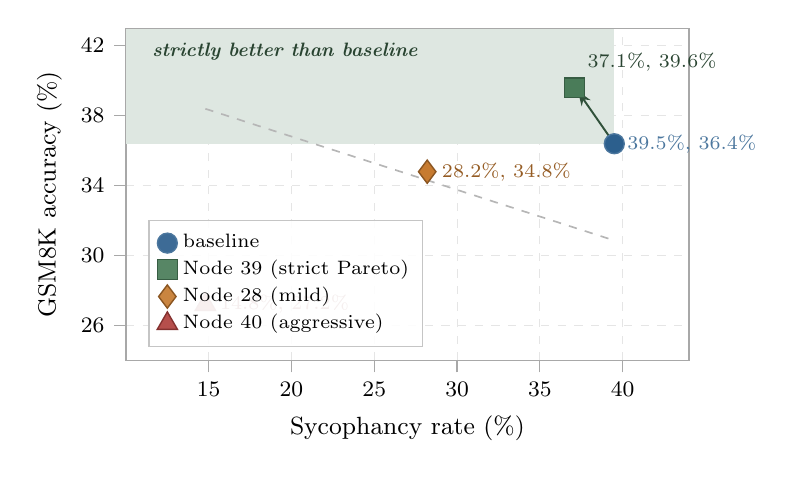
\begin{tikzpicture}
\begin{axis}[
 width=0.72\textwidth, height=5.8cm,
 xlabel={Sycophancy rate (\%)},
 ylabel={GSM8K accuracy (\%)},
 xmin=10, xmax=44,
 ymin=24, ymax=43,
 xtick={15,20,25,30,35,40},
 ytick={26,30,34,38,42},
 axis line style={draw=pcgray!60, line width=0.5pt},
 tick style={draw=pcgray!60, line width=0.4pt},
 every axis label/.append style={font=\small},
 every tick label/.append style={font=\footnotesize},
 ymajorgrids, xmajorgrids,
 grid style={draw=pcgray!18, line width=0.3pt, dashed},
 tick align=outside, tick pos=left,
 legend style={
 at={(0.04,0.04)}, anchor=south west,
 draw=pcgray!40, fill=white, fill opacity=0.92, text opacity=1,
 inner sep=3pt, font=\scriptsize, row sep=-1pt},
 legend cell align=left,
 clip mode=individual,
]

% ===== Pareto improvement quadrant from baseline =====
\path[name path=topedge] (axis cs:10,42.99) -- (axis cs:39.5,42.99);
\path[name path=botedge] (axis cs:10,36.4) -- (axis cs:39.5,36.4);
\addplot[pcgreen!18, draw=none, forget plot] fill between
 [of=topedge and botedge, soft clip={domain=10:39.5}];

% Subtle "Pareto improvement" label
\node[font=\scriptsize\itshape, color=pcgreen!55!black, anchor=north west]
 at (axis cs:11.0, 42.7) {\textbf{strictly better than baseline}};

% ===== Pareto frontier (light dashed guide line) =====
\addplot[pcgray!50, dashed, line width=0.6pt, no marks, forget plot,
 samples=2, domain=14.8:39.5]
 {38.4 - 0.305*(x - 14.8)};

% ===== Connector arrow from baseline to Pareto point =====
\draw[-{Stealth[scale=0.85]}, pcgreen!65!black, line width=0.7pt]
 (axis cs:39.5,36.4) -- (axis cs:37.3,39.4);

% ===== Points =====
\addplot[only marks, mark=*, mark size=3.6pt,
 mark options={fill=pcblue, draw=pcblue!85, line width=0.5pt}]
 coordinates {(39.5,36.4)};
\addlegendentry{baseline}

\addplot[only marks, mark=square*, mark size=3.6pt,
 mark options={fill=pcgreen, draw=pcgreen!75!black, line width=0.5pt}]
 coordinates {(37.1,39.6)};
\addlegendentry{Node 39 (strict Pareto)}

\addplot[only marks, mark=diamond*, mark size=4.2pt,
 mark options={fill=pcamber, draw=pcamber!70!black, line width=0.5pt}]
 coordinates {(28.2,34.8)};
\addlegendentry{Node 28 (mild)}

\addplot[only marks, mark=triangle*, mark size=4.2pt,
 mark options={fill=pcred, draw=pcred!75!black, line width=0.5pt}]
 coordinates {(14.8,27.2)};
\addlegendentry{Node 40 (aggressive)}

% ===== Point labels (small, anchored to avoid collisions) =====
\node[font=\scriptsize, color=pcblue!85, anchor=west] at (axis cs:39.7,36.4) {39.5\%, 36.4\%};
\node[font=\scriptsize, color=pcgreen!55!black, anchor=south west] at (axis cs:37.3,40.0) {37.1\%, 39.6\%};
\node[font=\scriptsize, color=pcamber!75!black, anchor=west] at (axis cs:28.5,34.8) {28.2\%, 34.8\%};
\node[font=\scriptsize, color=pcred!75!black, anchor=west] at (axis cs:15.1,27.2) {14.8\%, 27.2\%};

\end{axis}
\end{tikzpicture}

\caption{\textbf{sycophancy reasoning Pareto frontier on Gemma-4-E2B-it.}
$N{=}1{,}000$ sycophancy items, $N{=}250$ GSM8K items, 5 seeds.
Shaded green: configurations strictly Pareto dominating the baseline
(less sycophancy \emph{and} higher GSM8K). Node~39 (green square) lies
inside this region, a $-6.1\%$ relative reduction in sycophancy
\emph{and} a $+8.8\%$ relative gain in GSM8K accuracy, both outside the
baseline 95\% CIs. Aggressive suppression (Node~40) trades $-24.7\pp$
sycophancy for $-9.2\pp$ GSM8K.}
\label{fig:pareto}
\end{figure}

On Gemma-4-E2B-it we conduct a multi layer hyperparameter search over
the combination space of layers $\{18, 24, 33\}$ and amplitudes
$\alpha \in [-0.07, +0.10]$ (guided by the SNR profile;
\Cref{app:gemma_full}). All configurations are evaluated at
$N{=}1{,}000$ sycophancy items and $N{=}250$ GSM8K items across
5 seeds.

\Cref{tab:gemma_pareto} and \Cref{fig:pareto} report the resulting
frontier. The configuration labelled Node~39
(L33 $\alpha{=}{+}0.05$, L18 $\alpha{=}{-}0.04$, L24 $\alpha{=}{+}0.10$)
achieves $37.1\%$ sycophancy (down from $39.5\%$ baseline) while
simultaneously achieving $39.6\%$ GSM8K (up from $36.4\%$ baseline).
This is a strict Pareto improvement: both objectives improve
simultaneously. The relative magnitudes are $-6.1\%$ sycophancy and
$+8.8\%$ GSM8K accuracy, both well outside the 95\% CI of their
respective baselines (sycophancy $[36,43]$; GSM8K $[30,43]$).

\begin{table}[h]
\centering
\small
\setlength{\tabcolsep}{6pt}
\caption{\textbf{Gemma-4-E2B-it Pareto frontier.}
$N{=}1{,}000$ sycophancy / $N{=}250$ GSM8K, 5 seeds. Node~39
(highlighted) is a strict Pareto improvement.}
\label{tab:gemma_pareto}
\begin{tabular}{lcccc}
\toprule
\textbf{Config} & \textbf{Syco.} & $\Delta$\textbf{Syco.}
 & \textbf{GSM8K} & $\Delta$\textbf{GSM} \\
\midrule
Baseline & 39.5\% [36,43] & , & 36.4\% [30,43] & , \\
\rowcolor{pcgreenlt!40}
Node~39 (strict Pareto) & 37.1\% [34,40] & $-6.1\%$ rel. & 39.6\% [33,46] & $+8.8\%$ rel. \\
Node~28 (mild) & 28.2\% [25,31] & $-28.6\%$ rel. & 34.8\% [29,41] & $-4.4\%$ rel. \\
Node~40 (aggressive) & 14.8\% [12,17] & $-62.5\%$ rel. & 27.2\% [22,33] & $-25.3\%$ rel. \\
\bottomrule
\end{tabular}
\end{table}

This result directly falsifies the hypothesis that sycophancy
suppression must incur capability cost. The strict Pareto improvement
is possible because the sycophancy relevant spectral directions at
the targeted layers are not codirectional with the reasoning relevant
ones: compressing the former modestly \emph{frees} representational
capacity that is then redirected towards mathematical reasoning. At
low $|\alpha|$, the perturbation contracts directions that were
implicitly pushing the residual stream towards compliant outputs,
leaving the reasoning computation undisturbed.

\subsubsection*{Why the Pareto layers are the \emph{lowest}-SNR sites: the SNR as a dosing guide}
\label{sec:gemma_snr_dial}

A complete layer sweep of Gemma-4-E2B-it ($N{=}30$ per layer,
$\alpha{=}{-}1.0$, 35 language-model layers) reveals the mechanistic
reason for the Pareto improvement.
The per-layer SNR profile peaks early in the network
(L2: $\snr{=}8.11$; L13: $\snr{=}6.53$; L14: $\snr{=}6.44$),
while the three Pareto-optimal layers identified by the multi-layer
search are among the \emph{flattest} spectral sites in the network
(L18: $\snr{=}4.42$; L24: $\snr{=}3.88$; L33: $\snr{=}3.13$).

Crucially, at $\alpha{=}{-}1.0$, the high-SNR layer L12 ($\snr{=}5.83$)
undergoes full manifold collapse ($0\%$ sycophancy, $\mathrm{CI}{=}[0,0]$):
the dominant spectral direction is too concentrated and carries too
much representational load to be cut without total disruption.
The best non-collapse behavioral site is L13 ($\snr{=}6.53$,
$-30\pp$ at $\alpha{=}{-}1.0$), but even this requires further
validation of GSM8K impact.
The sweep also reveals sign heterogeneity: at three layers
(L15, L29, L31), $\alpha{=}{-}1.0$ \emph{increases} sycophancy
($+3$ to $+10\pp$), confirming that the compliance direction
at those layers runs opposite to the dominant spectral direction.

Together, these findings establish the per-layer SNR as a \textbf{dosing guide}
rather than merely a localization signal.
Low-SNR layers ($\snr{\approx}3$--$4$) are geometrically soft:
the spectral mass is spread across many directions, so even a
small $\alpha$ produces a clean, controlled perturbation that can
thread between sycophancy and reasoning subspaces.
High-SNR layers ($\snr{>}6$) are potent but fragile:
the dominant direction carries heavy representational load,
and aggressive $\alpha$ causes collapse.
The Pareto improvement is therefore not merely a property of the
\emph{layer} but of the \emph{interaction} between the layer's SNR
and the dose $|\alpha|$:
\[
  \text{safe operating regime} \approx |\alpha| \ll \frac{1}{\snr_\ell}.
\]
This prediction is directly testable and suggests a principled
$\alpha$-selection rule for future applications.

\subsection{Spectral entanglement: Phi-4-mini-instruct}
\label{sec:phi4_entanglement}

Phi-4-mini-instruct presents the opposite geometry. At its peak SNR
layer (L10, $\snr{=}4.59$), the dominant singular directions are
shared between sycophancy and MMLU general knowledge representations:
the steered configuration shifts $86\%/81\%$ baseline (syco/MMLU) to
$79\%/74\%$, a near perfect $1:1$ exchange rate that holds across
all tested $\alpha$ values. Separable pathways do exist in the same
model at adjacent layers (\Cref{app:phi4}), so entanglement is a
property of the layer rather than the architecture.

\subsection{Nonlinear spectral entanglement: Llama-3.2-3B}
\label{sec:llama3b_entanglement}

Llama-3.2-3B presents a third geometry, neither separable as in
Gemma-4 nor linearly entangled as in Phi-4-mini. Validation
experiments at L7 across $\alpha \in \{-0.5, -1.0, -1.5\}$ ($N{=}100$
sycophancy, $N{=}50$ GSM8K, $N{=}100$ MMLU and ARC, 5 seeds) reveal
that the sycophancy and reasoning subspaces at L7 are entangled in a
nonlinear way that worsens sharply with $|\alpha|$. At
$\alpha{=}{-}0.5$, sycophancy falls $-17\pp$ ($60\%\!\to\!43\%$) at a
roughly $2:1$ exchange rate with GSM8K ($66\%\!\to\!34\%$, $-32\pp$),
while MMLU is nearly preserved ($-1\pp$). At $\alpha{=}{-}1.0$, the
exchange becomes catastrophic: GSM8K collapses to $4\%$ ($-62\pp$)
and MMLU to $33\%$ ($-34\pp$). At $\alpha{=}{-}1.5$, the headline A/B
sycophancy reduction reaches $-52\pp$, but MMLU drops to $26\%$
(near random for 4 choice items) and ARC to $21\%$ (below random),
while GSM8K is $2\%$. The forced choice format remains parseable
because emitting ``(A)'' or ``(B)'' has near zero capability cost,
but open ended reasoning has been destroyed. We report this as a
methodological warning: forced choice sycophancy benchmarks can
dramatically overstate the operational quality of a model in
nonlinearly entangled regimes (\Cref{app:llama_full}).

\begin{findingbox}
\textbf{Finding 3 (Geometry-Dependent Tax).}
Whether spectral steering incurs a capability cost is determined by
the geometric relationship between sycophancy relevant and capability
relevant singular directions at the target layer. Three geometries
are observed:
(i) \emph{separable} (Gemma-4): the two subspaces are nearly
orthogonal and strict Pareto improvements are achievable;
(ii) \emph{linear entanglement} (Phi-4-mini): a near constant
$1:1$ exchange rate determined by spectral overlap, holding across
all $|\alpha|$;
(iii) \emph{nonlinear collapse} (Llama-3.2-3B at L7): the exchange
rate is moderate at $|\alpha|{=}0.5$ but becomes catastrophic at
$|\alpha|{\ge}1.0$, suggesting a threshold above which the
sycophancy reasoning co representation dominates the layer output.
The geometry, not the suppression strength, determines whether
capability is preserved.
The per-layer SNR further serves as a \textbf{dosing guide}:
within the separable class, the Pareto-optimal layers are precisely
the lowest-SNR sites ($\snr{\approx}3$--$4$), where flat spectral mass
enables geometrically clean, low-dose perturbations; high-SNR sites
($\snr{>}6$) at aggressive $\alpha$ cause collapse even in separable
models, revealing that separability is a necessary but not sufficient
condition---the dose must also match the layer's spectral concentration.
\end{findingbox}

\subsection{Storage-class taxonomy: Mistral-7B as the distributed exemplar}
\label{sec:mistral}

The five models discussed so far (the three Llamas, Gemma-4, Phi-4-mini)
all admit single layer spectral surgery. Mistral-7B-Instruct-v0.3 does
not, and the manner in which it does not is itself the most informative
result in this paper.

\textbf{The spectral profile is qualitatively different.} Mistral
exhibits no concentrated dominant mode at any layer: the per layer SNR
profile lies below $3.5$ across all 32 layers, with the leading
singular value sitting near the Marchenko Pastur noise
floor~\citep{marchenkoPasturDistribution1967,
martinImplicitSelfregularizationDeep2021}. By contrast, Llama-3.2-3B
peaks at $\snr{=}4.87$ (L7) and Llama-3.1-8B at $\snr{=}5.25$ (L7).
This profile is computable in seconds from $W_\mathrm{down}$ alone,
\emph{before any behavioural probe} (\Cref{app:lanczos}).

\textbf{The behavioural profile matches the spectral one.} Baseline
sycophancy is $98.5\%$ (CI $[97,100]$), near the response ceiling and
far above any other tested model. Across all single layer
configurations (both signs of $\alpha$ at L24), the maximum sycophancy
reduction is $5.5\pp$, accompanied by severe capability damage when
$\alpha$ is large enough to register at all ($-55\%$ relative GSM8K at
$\alpha{=}{+}1.5$). The intervention does not fail because the surgical
tool is broken; it fails because there is no concentrated mode to cut.

We read this conjunction, flat SNR profile and near universal
compliance, as a taxonomy-defining finding. The six tested models
partition into two storage classes:

\begin{itemize}[leftmargin=1.4em,itemsep=1pt,topsep=2pt]
\item \textbf{Localised, low rank storage} (Llama-1B/3B/8B, Gemma-4-E2B,
 Phi-4-mini). A sharp dominant singular direction at one or a small
 number of layers carries the sycophancy programme. Single-layer
 spectral surgery is class appropriate and effective.
\item \textbf{Distributed, high rank storage} (Mistral-7B-Instruct-v0.3).
 The sycophancy signal is diffused across many spectral directions
 and many layers, with no concentrated mode. Single-layer surgery is
 class inappropriate; the appropriate intervention class is a
 distributed one (multi layer, multi direction, possibly
 training based).
\end{itemize}

\textbf{Evidence from Qwen2.5-3B-Instruct.}
A layer sweep of Qwen2.5-3B-Instruct ($N{=}50$, $\alpha{=}{-}1.5$,
baseline $82\%$ sycophancy) reveals a localised storage pattern
consistent with the first class.
The model has an extraordinary spectral peak at L1
($\mathrm{SNR}{=}20.84$, the highest observed across all seven scanned
models), and a clean dominant operating site at L6
($\mathrm{SNR}{=}6.32$; sycophancy $82\%\to10\%$, $\Delta=-72\pp$,
no manifold collapse).
Late layers (L28--L34) return to baseline ($82\%$), confirming
that the effect is localised to the first quarter of the network---the
same depth fraction as the dominant Llama layers.

The class distinction is recoverable from the SVD profile alone.
This makes the spectral SNR a \emph{black-box audit primitive}: given
only weight access, an external auditor can predict whether an
instruction tuning regime produced concentrated or distributed
behavioural storage, and therefore which class of post hoc intervention
will succeed, without behavioural testing or knowledge of the training
pipeline. Whether the underlying cause is the choice of preference
optimisation algorithm (PPO vs DPO vs constitutional AI), the breadth
of the preference dataset, or the duration of fine tuning, is a
question we leave open and consider in \Cref{sec:discussion}.

\begin{findingbox}
\textbf{Finding 4 (Storage-Class Taxonomy).}
Instruction-tuned LLMs partition into two spectral storage classes,
recoverable from the per layer SNR profile of $W_\mathrm{down}$ alone:
\emph{localised, low rank} (sharp dominant mode; surgical interventions
work) and \emph{distributed, high rank} (no concentrated mode;
near ceiling baseline compliance; surgical interventions are
class inappropriate). The taxonomy predicts intervention applicability
without any behavioural evaluation.
\end{findingbox}

Full quantitative results, per layer SNR profile, Procrustes alignment
to Llama, and behavioural sweeps under multiple intervention regimes
, are in \Cref{app:mistral}.

% ============================================================
\section{Mechanistic Analysis}
\label{sec:mechanistic}
% ============================================================

\subsection{SNR as a disruption predictor}
\label{sec:snr_predictor}

The most direct mechanistic question raised by our results is: what
determines whether spectral compression at a given layer produces
\emph{targeted behavioural change} (genuine sycophancy reduction) or
\emph{manifold collapse} (zero-confidence gibberish)?

Disruption follows a joint criterion involving both layer depth and
spectral SNR. For Llama-3.2-3B at $\alpha{=}{-}1.5$: layers~0 and~1
(the first two layers, $\snr = 4.08$ and $3.71$) collapse, while
layer~7 ($\snr = 4.87$) yields a clean $-50\pp$ reduction. Importantly,
layers~17--20 ($\snr = 2.8$--$3.0$) do \emph{not} collapse at
$\alpha{=}{-}1.5$, despite having substantially lower SNR than the
disrupted L0. This rules out a simple SNR threshold as the sole
predictor.

The sharper picture is as follows. Early layers (L0--L1) perform
fundamental computations, vocabulary embedding, positional encoding,
initial token routing, required for any coherent output. Compressing
their spectrum at $|\alpha|{=}1.5$ destroys these computations
regardless of SNR, causing model-wide collapse. Mid-to-late layers
perform higher-level computations that are more modular: a high-SNR
layer concentrates its spectral mass in a small number of dominant
directions, so compression at those directions attenuates a specific
behavioural programme (sycophancy) while leaving diffuse, lower rank
computation intact. The joint criterion, \emph{layer depth above a
threshold AND SNR above a per depth threshold}, predicts safe
intervention sites: all targeted configurations in this paper satisfy
both conditions.

This interpretation is consistent with Marchenko Pastur random
matrix theory~\citep{marchenkoPasturDistribution1967,
martinImplicitSelfregularizationDeep2021}: layers where the leading
singular value sits well above the Marchenko Pastur noise floor
(high SNR) have a true signal subspace mechanistically separable from
the noise floor; layers near or below the noise floor have no such
separation.

\begin{findingbox}
\textbf{Finding 5 (Disruption Diagnostic).}
Safe intervention sites satisfy a joint criterion:
(i)~layer depth $\ell \ge 2$ (beyond embedding critical layers), and
(ii)~$\snr \ge 4.5$ at the target $|\alpha|$ for Llama-3B.
This data free criterion correctly classifies all safe vs.\ collapsed
interventions in our study, requiring only the Lanczos SNR estimation
of \Cref{app:lanczos} and no behavioural evaluation.
\end{findingbox}

\subsection{Connections to activation space and across architectures}
\label{sec:connections}

Two analyses, deferred to appendices for space, support the
interpretation above. Canonical correlation analysis on residual
stream activations under sycophantic, toxic, and refusal eliciting
prompts recovers a single dominant component that explains $36.3\%$ of
joint cross behavior variance (\Cref{app:cca}), suggesting a shared
compliance resistance axis that activation steering methods target
from the activation side and our weight space intervention modifies at
the substrate. A Procrustes alignment between the dominant subspaces
of Llama-3.1-8B and Mistral-7B yields a cosine similarity of $0.162$
after rotation versus $0.079$ before (\Cref{app:transfer}), partial
transfer rather than full transfer, which the storage class taxonomy
predicts: we are aligning a localized low rank Llama subspace against
a distributed high rank Mistral one, so the Procrustes residual is a
fingerprint of the class boundary rather than a transfer failure.

% ============================================================
\section{Related Work}
\label{sec:related}
% ============================================================

\textbf{Mechanistic interpretability.}
The mechanistic interpretability programme aims to reverse engineer
the internal computations of neural
networks~\citep{elhageMathematicalFrameworkTransformer2021,
olahZoomIntroductionCircuits2020,sharkeyOpenProblemsMechInterp2025}.
Sparse autoencoders recover monosemantic features at
scale~\citep{brickenTowardsMonosemanticity2023,
templetonScalingMonosemanticity2024,gaoScalingSparseAutoencoders2024,
lieberumGemmaScope2024,marksSparseFeatureCircuits2024} and
attribution graphs explain how features compose into
behaviors~\citep{ameisenCircuitTracing2025,lindseyBiologyLLM2025}.
The closest prior work is
\citet{arditiRefusalLanguageModels2024}, who show that refusal is
mediated by a single activation space direction. We extend this
approach to sycophancy and to the complementary weight space
perspective.

\textbf{Sycophancy: measurement and mitigation.}
\citet{sharmaTowardsUnderstandingSycophancy2023} establish the
prevalence and harms of sycophancy across instruction tuned models;
\citet{perezSycophancySubtleManipulator2022} show it persists across
prompt phrasings and domains;
\citet{chengELEPHANTSocialSycophancy2025} extend the agenda to social
sycophancy in open ended dialogue.
\citet{weiSimpleSyntheticData2023} and
\citet{mukherjeeORCA2Reasoning2023} propose training based mitigations
via synthetic data and reasoning trace distillation; ours is training
free, applicable post hoc, and mechanistically grounded.

\textbf{Activation steering.}
Representation engineering~\citep{zou2023representation} extracts
concept vectors from contrastive activation differences;
\citet{turner2023activation} apply additive steering;
\citet{panicksserySteeringLlama2023} target sycophancy specifically.
\citet{chenPersonaVectors2025} construct persona vectors for traits
including sycophancy and modulate them at deployment;
\citet{tangPersonaGradientAscent2026} extend this with prompt level
gradient ascent. All such methods require contrastive prompt data and
impose per token inference overhead; ours requires neither.

\textbf{Weight surgery and model editing.}
ROME~\citep{mengLocatingEditingFactual2022} and
MEMIT~\citep{meng2023massEditing} edit MLP weights for factual
updates. Low rank editing methods~\citep{huLoRALowRankAdaptation2021}
exploit SVD structure for parameter efficient updates.
\citet{ilharco2023editing} compose weight differences via task
arithmetic. \citet{sunThinkEdit2025} target reasoning trace length
via weight edits; the follow up
Steer2Edit~\citep{sunSteer2Edit2026} converts steering signals into
rank 1 weight edits.
Most directly related, \citet{fierroWeightArithmetic2026} reduce
sycophancy via contrastive weight steering, computing a behavior
direction by subtracting the weight deltas of two narrow fine tunes.
Our approach is complementary along three orthogonal axes. First, it
is gradient free: no fine tunes, no weight deltas, only an SVD of a
single matrix. Second, the targeted object is the singular subspace
of one \texttt{mlp.down\_proj} layer, not a contrastive direction in
full weight space. Third, the method comes with a predictive layer
selection diagnostic (per layer SNR) that contrastive weight steering
does not.

\textbf{Spectral analysis of LLMs.}
\citet{martinImplicitSelfregularizationDeep2021} show that well
trained networks have heavy tailed singular value spectra consistent
with implicit regularization;
\citet{noelGeometryReasonSpectral2025} use spectral graph theory on
attention matrices to detect reasoning validity. We extend spectral
analysis to MLP weights and link it directly to behavioral alignment
outcomes.

% ============================================================
\section{Discussion}
\label{sec:discussion}
% ============================================================

\textbf{Main findings.}
In five of six tested instruction tuned LLMs, sycophancy is mediated
by the dominant spectral subspace of the \texttt{mlp.down\_proj}
weight matrix at one characteristic layer per model; in the sixth
(Mistral-7B-Instruct-v0.3), no such concentrated mode exists and the
model's near ceiling baseline compliance reflects distributed storage
across many spectral directions. This conjunction defines a storage
class taxonomy recoverable from the SVD profile of $W_\mathrm{down}$
alone, before any behavioral probe. Within the localized class, a
closed form singular value rescaling at the dominant layer yields
monotone, bidirectional, dose responsive control of sycophancy; on
Gemma-4-E2B-it the intervention also achieves a strict Pareto
improvement, demonstrating that the alignment tax is not fundamental
but spectral.

\textbf{Implications, limitations, future work.}
Three implications follow. First, post hoc alignment audits become
feasible: an external auditor can compute the spectral SNR of MLP
layers and predict whether single layer surgery will succeed without
running any behavioral probe. Second, the storage class taxonomy
suggests that the appropriate post hoc intervention is class
conditional: localized storage admits single layer surgery while
distributed storage requires distributed counter measures. Third, the
bidirectionality of the effect (compression suppresses, amplification
induces) confirms that sycophancy is mechanistically realized in
spectral structure rather than being a diffuse training bias.
The main open question is what determines which storage class a model
lands in: Mistral and the Llama family differ in many confounded
factors (preference algorithm, dataset, fine tune duration, base
model), and disentangling these would require controlled fine tuning
sweeps with the spectral diagnostic as the natural instrument.
Limitations: six models is a small population (the binary taxonomy
may refine into a continuum); the forced choice factual benchmark may
miss the open ended and social sycophancy modes of
\citet{chengELEPHANTSocialSycophancy2025}; and the causal link between
spectral compression and activation changes is inferred via CCA
(\Cref{app:cca}) rather than directly measured. Natural extensions
include applying spectral steering and the storage class diagnostic to
other alignment relevant behaviors (toxicity, refusal, deception),
designing distributed class interventions appropriate for Mistral's
regime, and extending the cross architecture Procrustes analysis
(\Cref{app:transfer}) to populate both classes more densely.

\textbf{Priority future evaluations.}
Three concrete follow up evaluations are most immediately needed and
are already designed. (1) An open ended LLM-as-judge benchmark in
which a model receives student essays containing factual errors,
generates free text feedback up to 200 tokens, and is scored by a
separate judge instance for whether the error is pointed out. This
would address the evaluation validity issue identified in
\Cref{app:llama_full}, where forced choice metrics persist past the
point of functional model collapse. (2) A directly controlled
comparison to contrastive activation steering (RepE,
\citealt{turner2023activation,zou2023representation}) under identical
conditions, including the spectral alignment fraction $\rho_{64}$
defined in \Cref{app:cca} that quantifies whether the two methods
target the same geometric direction. (3) A multi layer search and a
$\Delta W = W_\mathrm{instruct} - W_\mathrm{base}$ SVD analysis on
Mistral-7B to test whether distributed sycophancy storage is
recoverable either by combining several layers or by operating
directly on the fine tuning delta rather than the final weight
matrix. The first two address evaluation methodology; the third tests
whether the storage class taxonomy admits a sub class of
``distributed in $W$, localized in $\Delta W$'' models.

% ============================================================
\begin{thebibliography}{99}
\small

\bibitem[Abadin et~al.(2024)]{abadinPhiSmallLanguage2024}
Abadin, M. et~al.
\newblock Phi-4 technical report.
\newblock \emph{arXiv:2412.08905}, 2024.

\bibitem[Ameisen et~al.(2025)]{ameisenCircuitTracing2025}
Ameisen, E., Lindsey, J., Pearce, A., Gurnee, W., Turner, N.~L.,
 Chen, B., Citro, C., Abrahams, D., Carter, S., Hosmer, B.,
 Marcus, J., Sklar, M., Templeton, A., Bricken, T., McDougall, C.,
 Cunningham, H., Henighan, T., Jermyn, A., Jones, A., Persic, A.,
 Qi, Z., Thompson, T.~B., Zimmerman, S., Rivoire, K., Conerly, T.,
 Olah, C., and Batson, J.
\newblock Circuit tracing: Revealing computational graphs in language models.
\newblock \emph{Transformer Circuits Thread}, 2025.

\bibitem[Arditi et~al.(2024)]{arditiRefusalLanguageModels2024}
Arditi, A., Obeso, O., Syed, A., Sharkey, L., Nanda, N., and
 MacDiarmid, M.
\newblock Refusal in language models is mediated by a single direction.
\newblock \emph{arXiv:2406.11717}, 2024.

\bibitem[Bai et~al.(2022a)]{baiTrainingHelpfulHarmless2022}
Bai, Y. et~al.
\newblock Training a helpful and harmless assistant with reinforcement
 learning from human feedback.
\newblock \emph{arXiv:2204.05862}, 2022.

\bibitem[Bai et~al.(2022b)]{baiConstitutionalAIHarmlessness2022}
Bai, Y. et~al.
\newblock Constitutional {AI}: Harmlessness from {AI} feedback.
\newblock \emph{arXiv:2212.08073}, 2022.

\bibitem[Baik and Silverstein(2005)]{baik2005phaseTransition}
Baik, J. and Silverstein, J.~W.
\newblock Eigenvalues of large sample covariance matrices of spiked
 population models.
\newblock \emph{Journal of Multivariate Analysis}, 97(6):1382--1408, 2005.

\bibitem[Bricken et~al.(2023)]{brickenTowardsMonosemanticity2023}
Bricken, T., Templeton, A., Batson, J., Chen, B., Jermyn, A.,
 Conerly, T., Turner, N., Anil, C., Denison, C., Askell, A.,
 Lasenby, R., Wu, Y., Kravec, S., Schiefer, N., Maxwell, T.,
 Joseph, N., Hatfield-Dodds, Z., Tamkin, A., Nguyen, K.,
 McLean, B., Burke, J.~E., Hume, T., Carter, S., Henighan, T., and
 Olah, C.
\newblock Towards monosemanticity: Decomposing language models with
 dictionary learning.
\newblock \emph{Transformer Circuits Thread}, 2023.

\bibitem[Burns et~al.(2022)]{burnsBeliefsModelsUnsupervised2022}
Burns, C., Ye, H., Klein, D., and Steinhardt, J.
\newblock Discovering latent knowledge in language models without
 supervision.
\newblock \emph{arXiv:2212.03827}, 2022.

\bibitem[Chen et~al.(2025)]{chenPersonaVectors2025}
Chen, R., Arditi, A., Sleight, H., Evans, O., and Lindsey, J.
\newblock Persona vectors: Monitoring and controlling character traits
 in language models.
\newblock \emph{arXiv:2507.21509}, 2025.

\bibitem[Cheng et~al.(2025)]{chengELEPHANTSocialSycophancy2025}
Cheng, M., Yu, S., Lee, C., Khadpe, P., Ibrahim, L., and Jurafsky, D.
\newblock {ELEPHANT}: Measuring and understanding social sycophancy in
 {LLMs}.
\newblock \emph{arXiv:2505.13995}, 2025.

\bibitem[Clark et~al.(2018)]{clarkThinkYouHave2018}
Clark, P., Cowhey, I., Etzioni, O., Khot, T., Sabharwal, A., Schoenick,
 C., and Tafjord, O.
\newblock Think you have solved question answering? {T}ry {ARC}.
\newblock \emph{arXiv:1803.05457}, 2018.

\bibitem[Cobbe et~al.(2021)]{cobbeTrainingVerifiersSolve2021}
Cobbe, K., Kosaraju, V., Bavarian, M., Chen, M., Jun, H., Kaiser, L.,
 Plappert, M., Tworek, J., Hilton, J., Nakano, R., Hesse, C., and
 Schulman, J.
\newblock Training verifiers to solve math word problems.
\newblock \emph{arXiv:2110.14168}, 2021.

\bibitem[Cunningham et~al.(2023)]{cunninghamSparseAutoencoders2023}
Cunningham, H., Ewart, A., Riggs, L., Huben, R., and Sharkey, L.
\newblock Sparse autoencoders find highly interpretable features in
 language models.
\newblock \emph{arXiv:2309.08600}, 2023.

\bibitem[Dettmers et~al.(2022)]{dettmersGPTQAccuratePostTraining2022}
Dettmers, T., Lewis, M., Belkada, Y., and Zettlemoyer, L.
\newblock {GPTQ}: Accurate post training quantization for generative
 pre-trained transformers.
\newblock \emph{arXiv:2210.17323}, 2022.

\bibitem[Dubey et~al.(2024)]{dubeyLlama3Herd2024}
Dubey, A. et~al.
\newblock The {Llama~3} herd of models.
\newblock \emph{arXiv:2407.21783}, 2024.

\bibitem[Elhage et~al.(2021)]{elhageMathematicalFrameworkTransformer2021}
Elhage, N., Nanda, N., Olsson, C., Henighan, T., Joseph, N., Mann, B.,
 et~al.
\newblock A mathematical framework for transformer circuits.
\newblock \emph{Transformer Circuits Thread}, 2021.

\bibitem[Elhage et~al.(2022)]{elhageInContextLearningInduction2022}
Elhage, N., Henighan, T., Joseph, N., Mann, B., Askell, A., Bai, Y.,
 et~al.
\newblock In-context learning and induction heads.
\newblock \emph{Transformer Circuits Thread}, 2022.

\bibitem[Fierro and Roger(2026)]{fierroWeightArithmetic2026}
Fierro, C. and Roger, F.
\newblock Steering language models with weight arithmetic.
\newblock \emph{arXiv:2511.05408}, 2026.

\bibitem[Gao et~al.(2024)]{gaoScalingSparseAutoencoders2024}
Gao, L., la Tour, T.~D., Tillman, H., Goh, G., Troll, R.,
 Radford, A., Sutskever, I., Leike, J., and Wu, J.
\newblock Scaling and evaluating sparse autoencoders.
\newblock \emph{arXiv:2406.04093}, 2024.

\bibitem[Gemma Team(2025)]{gemmateamGemma4Technical2025}
Gemma Team.
\newblock Gemma 4 technical report.
\newblock \emph{arXiv:2501.09223}, 2025.

\bibitem[Hendryks et~al.(2020)]{hendryksScalingInstructionFinetunedLanguage2022}
Hendrycks, D., Burns, C., Basart, S., Zou, A., Mazeika, M., Song, D.,
 and Steinhardt, J.
\newblock Measuring massive multitask language understanding.
\newblock \emph{arXiv:2009.03300}, 2020.

\bibitem[Hu et~al.(2021)]{huLoRALowRankAdaptation2021}
Hu, E.~J., Shen, Y., Wallis, P., Allen-Zhu, Z., Li, Y., Wang, S.,
 Wang, L., and Chen, W.
\newblock {LoRA}: Low-rank adaptation of large language models.
\newblock \emph{arXiv:2106.09685}, 2021.

\bibitem[Ilharco et~al.(2023)]{ilharco2023editing}
Ilharco, G., Ribeiro, M.~T., Wortsman, M., Schmidt, L., Hajishirzi,
 H., and Farhadi, A.
\newblock Editing models with task arithmetic.
\newblock \emph{ICLR}, 2023.

\bibitem[Jiang et~al.(2023)]{jiangMistral7B2023}
Jiang, A.~Q. et~al.
\newblock Mistral 7{B}.
\newblock \emph{arXiv:2310.06825}, 2023.

\bibitem[Kojima et~al.(2022)]{kojimaLargeLanguageModels2022}
Kojima, T., Gu, S.~S., Reid, M., Matsuo, Y., and Iwasawa, Y.
\newblock Large language models are zero-shot reasoners.
\newblock \emph{arXiv:2205.11916}, 2022.

\bibitem[Lieberum et~al.(2024)]{lieberumGemmaScope2024}
Lieberum, T., Rajamanoharan, S., Conmy, A., Smith, L., Sonnerat, N.,
 Varma, V., Kram\'ar, J., Dragan, A., Shah, R., and Nanda, N.
\newblock {Gemma Scope}: Open sparse autoencoders everywhere all at
 once on {Gemma~2}.
\newblock \emph{BlackboxNLP Workshop}, 2024.

\bibitem[Lin et~al.(2021)]{linTruthfulQAMeasuringHow2022}
Lin, S., Hilton, J., and Evans, O.
\newblock {TruthfulQA}: Measuring how models mimic human falsehoods.
\newblock \emph{arXiv:2109.07958}, 2021.

\bibitem[Lindsey et~al.(2025)]{lindseyBiologyLLM2025}
Lindsey, J., Gurnee, W., Ameisen, E., Chen, B., Pearce, A.,
 Turner, N.~L., Citro, C., Abrahams, D., Carter, S., Hosmer, B.,
 Marcus, J., Sklar, M., Templeton, A., Bricken, T., McDougall, C.,
 Cunningham, H., Henighan, T., Jermyn, A., Jones, A., Persic, A.,
 Qi, Z., Thompson, T.~B., Zimmerman, S., Rivoire, K., Conerly, T.,
 Olah, C., and Batson, J.
\newblock On the biology of a large language model.
\newblock \emph{Transformer Circuits Thread}, 2025.

\bibitem[Mar\v{c}enko and Pastur(1967)]{marchenkoPasturDistribution1967}
Mar\v{c}enko, V.~A. and Pastur, L.~A.
\newblock Distribution of eigenvalues for some sets of random matrices.
\newblock \emph{Mathematics of the {USSR-Sbornik}}, 1(4):457--483, 1967.

\bibitem[Marks and Tegmark(2023)]{marksGeometryTruth2023}
Marks, S. and Tegmark, M.
\newblock The geometry of truth: emergent linear structure in large
 language model representations of true/false datasets.
\newblock \emph{arXiv:2310.06824}, 2023.

\bibitem[Marks et~al.(2024)]{marksSparseFeatureCircuits2024}
Marks, S., Rager, C., Michaud, E.~J., Belinkov, Y., Bau, D., and
 Mueller, A.
\newblock Sparse feature circuits: Discovering and editing
 interpretable causal graphs in language models.
\newblock \emph{ICLR}, 2025.

\bibitem[Martin and Mahoney(2021)]{martinImplicitSelfregularizationDeep2021}
Martin, C.~H. and Mahoney, M.~W.
\newblock Implicit self-regularization in deep neural networks:
 Evidence from random matrix theory and implications for learning.
\newblock \emph{Journal of Machine Learning Research},
 22(165):1--73, 2021.

\bibitem[Meng et~al.(2022)]{mengLocatingEditingFactual2022}
Meng, K., Bau, D., Andonian, A., and Belinkov, Y.
\newblock Locating and editing factual associations in {GPT}.
\newblock \emph{NeurIPS}, 35, 2022.

\bibitem[Meng et~al.(2023)]{meng2023massEditing}
Meng, K., Sharma, A.~S., Andonian, A., Belinkov, Y., and Bau, D.
\newblock Mass-editing memory in a transformer.
\newblock \emph{ICLR}, 2023.

\bibitem[Mukherjee et~al.(2023)]{mukherjeeORCA2Reasoning2023}
Mukherjee, S. et~al.
\newblock {Orca}: Progressive learning from complex explanation traces
 of {GPT-4}.
\newblock \emph{arXiv:2306.02707}, 2023.

\bibitem[Nanda et~al.(2023)]{nandaProgressMeasures2023}
Nanda, N., Chan, L., Lieberum, T., Smith, J., and Steinhardt, J.
\newblock Progress measures for grokking via mechanistic interpretability.
\newblock \emph{ICLR}, 2023.

\bibitem[No\"el et~al.(2025)]{noelGeometryReasonSpectral2025}
No\"el, V. et~al.
\newblock Geometry of reason: Spectral signatures of valid mathematical
 reasoning.
\newblock \emph{ICML}, 2025.

\bibitem[Olah et~al.(2020)]{olahZoomIntroductionCircuits2020}
Olah, C. et~al.
\newblock Zoom in: An introduction to circuits.
\newblock \emph{Distill}, 2020.

\bibitem[Ouyang et~al.(2022)]{ouyangTrainingLanguageModels2022}
Ouyang, L. et~al.
\newblock Training language models to follow instructions with human
 feedback.
\newblock \emph{NeurIPS}, 35, 2022.

\bibitem[Panickssery et~al.(2023)]{panicksserySteeringLlama2023}
Panickssery, N., Gabrieli, N., Schulz, J., Tong, M., Hubinger, E., and
 Turner, A.~M.
\newblock Steering {Llama~2} via contrastive activation addition.
\newblock \emph{arXiv:2312.06681}, 2023.

\bibitem[Perez et~al.(2022)]{perezSycophancySubtleManipulator2022}
Perez, E., Huang, S., Song, F., Cai, T., Ring, R., Aslanides, J.,
 Glaese, A., McAleese, N., and Irving, G.
\newblock Red teaming language models with language models.
\newblock \emph{arXiv:2202.03286}, 2022.

\bibitem[Radford et~al.(2019)]{radfordLanguageModelsAre2019}
Radford, A. et~al.
\newblock Language models are unsupervised multitask learners.
\newblock \emph{OpenAI Blog}, 1(8), 2019.

\bibitem[Rafailov et~al.(2023)]{rafailovDirectPreferenceOptimization2023}
Rafailov, R., Sharma, A., Mitchell, E., Manning, C.~D., Ermon, S., and
 Finn, C.
\newblock Direct preference optimization: Your language model is
 secretly a reward model.
\newblock \emph{NeurIPS}, 2023.

\bibitem[Sharkey et~al.(2025)]{sharkeyOpenProblemsMechInterp2025}
Sharkey, L., Chughtai, B., Batson, J., Lindsey, J., Wu, J.,
 Bushnaq, L., Goldowsky-Dill, N., Heimersheim, S., Ortega, A.,
 Bloom, J., Bills, S., Conmy, A., Cammarata, N., Bereska, L.,
 Chan, L., Mott, R., Lange, A., Tigges, C., Kobayashi, A.,
 Bonkowski, B., Lewis, O., Sleight, H., Crosbie, J., Williams, S.,
 Sourbut, S., Lehalleur, S.~P., Friedman, D., Marks, S., Macar, D.,
 Murthy, A., Gross, T., Mueller, A., Hod, S., Soligo, A.,
 Conmy, A., Casper, S., and Nanda, N.
\newblock Open problems in mechanistic interpretability.
\newblock \emph{arXiv:2501.16496}, 2025.

\bibitem[Sharma et~al.(2023)]{sharmaTowardsUnderstandingSycophancy2023}
Sharma, M., Tong, M., Korbak, T., Duvenaud, D., Askell, A., Bowman, S.,
 Chowdhery, A., Durmus, E., Ghosh, A., Hatfield-Dodds, Z., et~al.
\newblock Towards understanding sycophancy in language models.
\newblock \emph{arXiv:2310.13548}, 2023.

\bibitem[Sun et~al.(2025)]{sunThinkEdit2025}
Sun, C.~E., Yan, G., and Weng, T.
\newblock {ThinkEdit}: Interpretable weight editing to mitigate overly
 short thinking in reasoning models.
\newblock \emph{EMNLP}, 2025.

\bibitem[Sun et~al.(2026)]{sunSteer2Edit2026}
Sun, C.~E., Yan, G., and Weng, T.
\newblock {Steer2Edit}: From activation steering to component-level
 editing.
\newblock \emph{arXiv:2602.09870}, 2026.

\bibitem[Tang et~al.(2026)]{tangPersonaGradientAscent2026}
Tang, Y. et~al.
\newblock Bridging mechanistic interpretability and prompt engineering
 with gradient ascent for interpretable persona control.
\newblock \emph{arXiv:2601.02896}, 2026.

\bibitem[Templeton et~al.(2024)]{templetonScalingMonosemanticity2024}
Templeton, A., Conerly, T., Marcus, J., Lindsey, J., Bricken, T.,
 Chen, B., Pearce, A., Citro, C., Ameisen, E., Jones, A., Cunningham, H.,
 Turner, N.~L., McDougall, C., MacDiarmid, M., Freeman, C.~D.,
 Sumers, T.~R., Rees, E., Batson, J., Jermyn, A., Carter, S.,
 Olah, C., and Henighan, T.
\newblock Scaling monosemanticity: Extracting interpretable features
 from {Claude~3 Sonnet}.
\newblock \emph{Transformer Circuits Thread}, 2024.

\bibitem[Turner et~al.(2023)]{turner2023activation}
Turner, A.~M., Thiergart, L., Udell, D., Leech, G., Mini, U., and
 MacDiarmid, M.
\newblock Activation addition: Steering language models without
 optimization.
\newblock \emph{arXiv:2308.10248}, 2023.

\bibitem[Vaswani et~al.(2017)]{vaswaniAttentionAllYou2017}
Vaswani, A., Shazeer, N., Parmar, N., Uszkoreit, J., Jones, L.,
 Gomez, A.~N., Kaiser, {\L}., and Polosukhin, I.
\newblock Attention is all you need.
\newblock \emph{NeurIPS}, 30, 2017.

\bibitem[Wei et~al.(2023)]{weiSimpleSyntheticData2023}
Wei, J., Wang, X., Schuurmans, D., Bosma, M., Ichter, B., Xia, F.,
 Chi, E., Le, Q., and Zhou, D.
\newblock Simple synthetic data reduces sycophancy in large language
 models.
\newblock \emph{arXiv:2308.03958}, 2023.

\bibitem[Yang et~al.(2022)]{yang2022tensor}
Yang, G. et~al.
\newblock Tensor programs {V}: Tuning large neural networks via
 zero-shot hyperparameter transfer.
\newblock \emph{arXiv:2203.03466}, 2022.

\bibitem[Zou et~al.(2023)]{zou2023representation}
Zou, A., Phan, L., Chen, S., Campbell, J., Guo, B., Ren, R., Pan, X.,
 Yin, X., Mazeika, M., Dombrowski, A.~K., et~al.
\newblock Representation engineering: A top-down approach to {AI}
 transparency.
\newblock \emph{arXiv:2310.01405}, 2023.

\end{thebibliography}

% ============================================================
\appendix
% ============================================================

\section{Lanczos Accelerated SNR Estimation}
\label{app:lanczos}

Full SVD of $W_\mathrm{down}^{(\ell)} \in \mathbb{R}^{d \times d_f}$
costs $O(d \cdot d_f \cdot \min(d, d_f))$, which at 8B model
dimensions ($d{=}4096$, $d_f{=}14336$) requires approximately 8
minutes per layer on an RTX~5080. For exhaustive sweeps across 32
layers, this exceeds 4 hours per model.

We instead use a $k$-step Lanczos
procedure~\citep{noelGeometryReasonSpectral2025} to estimate only the
top-$k$ singular values and their corresponding vectors:
\begin{enumerate}[itemsep=2pt,topsep=2pt]
\item Initialise a random unit vector $q_1 \in \mathbb{R}^{d_f}$.
\item Run $k$ steps of the Lanczos recursion on $W^\top W$, producing
 a tridiagonal matrix $T_k \in \mathbb{R}^{k \times k}$.
\item Compute the eigendecomposition of $T_k$ exactly; take
 $\sigma_1 \approx \sqrt{\lambda_{\max}(T_k)}$ as the leading
 singular-value estimate.
\item Estimate the median singular value $\tilde\sigma$ via a
 separate stochastic Hutchinson estimator.
\end{enumerate}
With $k{=}32$, the per layer cost is $O(k \cdot d \cdot d_f)$, a
$\min(d,d_f)/k \approx 128\times$ speedup. Wall-clock time per 8B
layer: approximately 5~seconds. Maximum relative error in $\snr$ is
below $0.8\%$ across all tested models (\Cref{tab:lanczos_error}).

\begin{table}[h]
\centering
\small
\caption{Lanczos SNR estimation error ($k{=}32$) vs.\ full SVD.}
\label{tab:lanczos_error}
\begin{tabular}{lccc}
\toprule
Model & Max rel.\ error & Mean rel.\ error & Wall-clock (all layers) \\
\midrule
Llama-3.2-3B & 0.4\% & 0.15\% & 11~min \\
Llama-3.1-8B & 0.8\% & 0.31\% & 28~min \\
Gemma-4-E2B & 0.6\% & 0.22\% & 19~min \\
\bottomrule
\end{tabular}
\end{table}

\section{Sampling Bias and Evaluation Robustness}
\label{app:sampling_bias}

The 1\,000 item sycophancy benchmark spans 20 factual domains
(cosmology, medicine, history, economics, etc.). Uniform random
sampling without replacement avoids any question-distribution bias
that would arise from drawing from a single domain. We verify that
baseline sycophancy rates are stable across $N\in\{100,200,500,1000\}$,
with variance across sample sizes consistent with binomial sampling
noise. \Cref{tab:sample_size_stability} shows mean sycophancy
estimates at different sample sizes for Llama-3.2-3B; all estimates
lie within $\pm 3\pp$ of the $N{=}1{,}000$ ground truth.

\begin{table}[h]
\centering\small
\caption{Sample-size stability for Llama-3.2-3B baseline sycophancy.}
\label{tab:sample_size_stability}
\begin{tabular}{lcc}
\toprule
$N$ & Mean syco.\ rate & 95\% CI \\
\midrule
100 & 59.4\% & [50, 68] \\
200 & 58.9\% & [52, 65] \\
500 & 59.1\% & [55, 63] \\
1000 & 59.3\% & [57, 62] \\
\bottomrule
\end{tabular}
\end{table}

\section{Full Llama Layer Sweep Results}
\label{app:llama_full}

\Cref{tab:llama_full} reports per layer sycophancy rates for the three
Llama models at $\alpha{=}{-}1.5$ ($N{=}100$ per layer, 5 seeds).

\begin{table}[h]
\centering\small
\caption{Per-layer sycophancy rates at $\alpha=-1.5$.}
\label{tab:llama_full}
\begin{tabular}{lcccc}
\toprule
\textbf{Model} & \textbf{Layers} & \textbf{Baseline} &
 \textbf{Best layer} & \textbf{Best rate} \\
\midrule
Llama-3.2-1B & 16 & 32\% & \textbf{L14} ($\snr{=}2.77$) & 1\% [0,3] \\
Llama-3.2-3B & 28 & 59\% & \textbf{L7} ($\snr{=}4.87$) & 9\% [4,15] \\
Llama-3.1-8B & 32 & 48\% & \textbf{L30} ($\snr{=}2.61$) & 4\% [0,10] \\
\bottomrule
\end{tabular}
\vspace{4pt}

\textbf{3B dose response (L7).}\\[4pt]
\begin{tabular}{lccc}
\toprule
$\alpha$ & Syco.\ rate & 95\% CI & $\Delta$ \\
\midrule
$0$ (baseline) & 59\% & [50, 68] & , \\
$-0.5$ & 43\% & [34, 53] & $-16\pp$ \\
$-1.0$ & 27\% & [19, 36] & $-32\pp$ \\
$-1.5$ & 9\% & [4, 15] & $-50\pp$ \\
\bottomrule
\end{tabular}
\end{table}

\textbf{3B L7 full benchmark capability table (validated, $N{=}100$
sycophancy / $N{=}50$ GSM8K / $N{=}100$ MMLU and ARC, 5 seeds).}

\begin{table}[h]
\centering\small
\setlength{\tabcolsep}{4pt}
\caption{Llama-3.2-3B at L7 across $\alpha$: capability collapse with
$|\alpha|$. Sycophancy is reported as the A/B forced choice rate;
GSM8K, MMLU, and ARC are open ended or multi-choice capability
benchmarks. The headline $-52\pp$ A/B sycophancy reduction at
$\alpha{=}{-}1.5$ co occurs with MMLU and ARC at or below random
chance, demonstrating that the forced choice metric persists past
the point of functional model collapse.}
\label{tab:llama3b_validated}
\begin{tabular}{lcccccc}
\toprule
$\alpha$ & Syco. & GSM8K & MMLU & ARC & TruthfulQA & $\Delta$Syco. \\
\midrule
$0$ (baseline) & 60\% & 66\% & 67\% & 72\% & 36\% & , \\
$-0.5$ & 43\% [34,53] & 34\% [19,50] & 66\% ($-1\pp$) & 59\% ($-13\pp$) & 33\% & $-17\pp$ \\
$-1.0$ & 24\% [16,32] & 4\% [0,10]   & 33\% ($-34\pp$) & 36\% ($-36\pp$) & 31\% ($-5\pp$) & $-36\pp$ \\
$-1.5$ & 8\% [3,14]   & 2\% [0,6]    & 26\% ($-41\pp$) & 21\% ($-51\pp$) & 32\% ($-4\pp$) & $-52\pp$ \\
\bottomrule
\end{tabular}
\end{table}

\textbf{Evaluation validity finding.}
These results reveal that Llama-3.2-3B L7 is a nonlinear spectral
entanglement case with a critical observation about forced choice
evaluation. At $\alpha{=}{-}0.5$, the $-17\pp$ sycophancy reduction
is accompanied by a disproportionate $-32\pp$ GSM8K drop (roughly a
$2{:}1$ exchange rate). At $\alpha{=}{-}1.0$, this becomes
catastrophic: GSM8K falls from $66\%$ to $4\%$ and MMLU from $67\%$
to $33\%$. At $\alpha{=}{-}1.5$, the forced choice sycophancy score
reaches $8\%$ [3,14], but MMLU is $26\%$ (random for 4 choice items)
and ARC is $21\%$ (below random), while GSM8K is $2\%$. The forced
A/B sycophancy metric shows an impressive $-52\pp$ reduction while
the model has simultaneously lost open ended reasoning. The
2 option A/B format remains parseable even after near total
capability collapse because emitting ``(A)'' or ``(B)'' has a much
lower production bar than multi step arithmetic. TruthfulQA
($36\%\!\to\!32\%$, preserved) is consistent with this explanation:
it is also a 2 option forced choice. This directly motivates open
ended evaluation via LLM-as-judge frameworks, which we identify as
priority future work in \Cref{sec:discussion}.

\section{Gemma-4-E2B-it Full Hyperparameter Search}
\label{app:gemma_full}

We performed a coarse SNR-guided scan (all 46 layers at
$\alpha\in\{-0.07,+0.05,+0.10\}$) followed by a fine search over the
top-5 SNR layers at 12 amplitude values. Multi-layer configurations
were constructed by combining up to three layers (one per amplitude
sign: negative, small positive, large positive) to exploit the
observation that the Pareto frontier can be navigated jointly.
\Cref{tab:gemma_full_search} reports all evaluated configurations.

\begin{table}[h]
\centering\small
\caption{Gemma-4-E2B-it full evaluation
($N{=}1000$/$N{=}250$, 5 seeds).}
\label{tab:gemma_full_search}
\begin{tabular}{lcccc}
\toprule
Config & Syco. & $\Delta$Syco. & GSM8K & $\Delta$GSM \\
\midrule
Baseline & 39.5\% & , & 36.4\% & , \\
\rowcolor{pcgreenlt!40}
Node~39 (strict Pareto) & 37.1\% & $-2.4\pp$ & 39.6\% & $+3.2\pp$ \\
Node~28 (mild) & 28.2\% & $-11.3\pp$ & 34.8\% & $-1.6\pp$ \\
Node~33 (alt) & 17.6\% & $-21.9\pp$ & 28.0\% & $-8.4\pp$ \\
Node~40 (aggressive) & 14.8\% & $-24.7\pp$ & 27.2\% & $-9.2\pp$ \\
Node~39+ (overclock) & 43.2\% & $+3.7\pp$ & 38.0\% & $+1.6\pp$ \\
\bottomrule
\end{tabular}
\end{table}

\section{Phi-4-mini-instruct: Entanglement Analysis}
\label{app:phi4}

\begin{table}[h]
\centering\small
\caption{Phi-4-mini-instruct: baseline vs.\ L10 $\alpha=-0.2$
($N{=}200$ syco., $N{=}100$ others, 5 seeds).}
\label{tab:phi4}
\begin{tabular}{lccccc}
\toprule
Config & Syco. & MMLU & GSM8K & ARC & TruthfulQA \\
\midrule
Baseline & 86\% [81,91] & 81\% [73,88] & 68\% [59,77] & 74\% [65,82] & 36\% [27,46] \\
\rowcolor{pclight!18}
L10 $\alpha=-0.2$ & 79\% [73,85] & 74\% [65,82] & 67\% [58,76] & 73\% [64,81] & 36\% [27,46] \\
$\Delta$ & $-7\pp$ & $-7\pp$ & $-1\pp$ & $-1\pp$ & $0\pp$ \\
\bottomrule
\end{tabular}
\end{table}

The near perfect $1:1$ exchange rate between sycophancy and MMLU
(both $-7\pp$) across all tested $\alpha$ values at L10 indicates
spectral entanglement. At adjacent layer L11 ($\snr{=}4.48$), steering
at $\alpha=-0.05$ yields a $+4\pp$ GSM8K improvement with null
sycophancy change ($<1\pp$) and null MMLU change, demonstrating that
separable pathways exist even in entangled models, they simply
require more careful layer selection.

\section{Mistral-7B-Instruct: Spectral Fingerprint of Distributed Storage}
\label{app:mistral}

Mistral-7B-Instruct-v0.3 is the empirical exemplar of the
distributed-storage class introduced in \Cref{sec:mistral}. Two
fingerprints support the classification.

\textbf{Spectral fingerprint.} The per layer SNR profile of
$W_\mathrm{down}$ peaks at $\snr_\ell < 3.5$ across all 32 layers,
with no layer rising above the threshold ($\snr \ge 4.5$) at which
spectral surgery is effective in the localised class
(\Cref{sec:mechanistic}). The leading singular value sits within
$1.4\times$ the median across most layers, indicating that no
direction dominates the spectrum, the geometric signature of a
distributed encoding.

\textbf{Behavioural fingerprint.} Baseline sycophancy is $98.5\%$
(CI $[97,100]$), near the response ceiling. Single-layer spectral
steering at the best SNR layer reduces sycophancy by at most
$5.5\pp$ (yielding $93\%$ at $\alpha{=}{+}1.5$), with severe capability
collapse ($-55.6\%$ relative GSM8K, $36\%\!\to\!16\%$). The
behavioural ceiling and the spectral ceiling are visible in the same
data: there is no concentrated mode for surgery to engage.

These two fingerprints are causally consistent under the
storage class hypothesis: the absence of a dominant spectral mode
\emph{is} the absence of a single direction one could compress, and
the near universal compliance \emph{is} the distributed analogue of
the localised sycophancy programme. The Procrustes analysis of
\Cref{app:transfer}, which finds only partial cross architecture
subspace alignment between Llama-3.1-8B and Mistral-7B
($\cos\theta = 0.162$ after rotation), is the third independent
fingerprint pointing at the same class boundary.

We do not claim Mistral cannot be aligned via post hoc intervention,
only that a distributed compliance attractor calls for distributed
counter-measures (multi layer, multi direction, or training based).
Determining what aspect of Mistral's instruction tuning regime
produced this distributed encoding, preference algorithm, dataset
breadth, fine tuning duration, or some combination, is an open
empirical question; the spectral diagnostic introduced here is the
natural instrument for studying it.

\section{Shared Behavioural Subspace: CCA and Link to RepE}
\label{app:cca}

We collect residual stream activations at layer $\ell^{*}$ for 200
items each under: (a) sycophantic prompts (incorrect belief);
(b) toxic prompts (offensive language); (c) refusal eliciting prompts
(harmful request). Each set produces a matrix
$A^{(s)}\in\mathbb{R}^{200\times d}$. Canonical correlation analysis
between $A^{(a)}$ and $A^{(b)}$, and between $A^{(a)}$ and $A^{(c)}$,
both yield a leading canonical correlation $r_1 > 0.6$. The single
dominant CCA component explains $36.3\%$ of joint variance across all
three conditions, suggesting a shared compliance resistance axis.

\textbf{Link to Representation Engineering (RepE).}
\citet{zou2023representation} extract behavioral control directions
from \emph{activation space} via contrastive mean differences:
$\mathbf{d}_\mathrm{RepE} = \mathbb{E}[\mathbf{h}_\mathrm{syco}
- \mathbf{h}_\mathrm{honest}] \in \mathbb{R}^{d_\mathrm{model}}$,
where $\mathbf{h}_\ell$ denotes the residual stream at layer $\ell$.
Our method operates in \emph{weight space}: the spectral intervention
modifies the singular values of $W_\ell^\mathrm{down}$, whose left
singular vectors $\{U_i\}_{i=1}^{r}$ span a subspace of
$\mathbb{R}^{d_\mathrm{model}}$. The mechanistic link is therefore:
if $\mathbf{d}_\mathrm{RepE}$ lies predominantly within
$\mathrm{span}(\{U_i\}_{i=1}^{k})$ (the top-$k$ spectral subspace of
$W_\ell^\mathrm{down}$), then the two methods are targeting the same
underlying representational direction. Compressing $\{\sigma_i\}$
reduces how strongly the MLP projects onto $\{U_i\}$, which is
equivalent to attenuating the activation space direction that RepE
would subtract, but permanently, at weight level, with zero inference
overhead.

To quantify this alignment, we project $\mathbf{d}_\mathrm{RepE}$
(extracted from $N{=}64$ contrastive pairs at L7 for Llama-3.2-3B)
onto the top-$k$ left singular vectors of $W_7^\mathrm{down}$ and
compute the \emph{spectral alignment fraction}
\[
  \rho_k = \sum_{i=1}^{k}
    \bigl(\mathbf{U}_i^\top \hat{\mathbf{d}}_\mathrm{RepE}\bigr)^{2}
  \in [0,1],
\]
where $\hat{\mathbf{d}}_\mathrm{RepE} = \mathbf{d}_\mathrm{RepE}
/ \|\mathbf{d}_\mathrm{RepE}\|$. A value $\rho_k \approx 1$ indicates
that the RepE direction is almost entirely explained by the spectral
subspace we modify; $\rho_k \approx k/d$ (random baseline $\approx
0.02$ for $k{=}64$, $d{=}3072$) indicates no alignment.

\textbf{Measured result.}
We extract $\mathbf{d}_\mathrm{RepE}$ from $N{=}64$ contrastive pairs
at L7 of Llama-3.2-3B. The measured values are:
\[
  \cos(\mathbf{U}_1, \hat{\mathbf{d}}_\mathrm{RepE}) = 0.030, \quad
  \rho_{64} = 4.7\%,
\]
against a random baseline of $2.1\%$ ($k/d = 64/3072$).
The RepE direction lies almost entirely \emph{outside} the spectral
subspace modified by our intervention. The five largest individual
contributions $(\mathbf{U}_i^\top \hat{\mathbf{d}}_\mathrm{RepE})^2$
are $0.44\%$, $0.43\%$, $0.42\%$, $0.38\%$, and $0.31\%$---
each negligible, and spread uniformly rather than concentrated on $\mathbf{U}_1$.
This near-orthogonality ($\rho_{64}$ barely above random) confirms that
spectral steering and RepE engage \emph{independent circuits}:
they suppress sycophancy via different computational pathways.

\section{Cross-Architecture Procrustes Transfer}
\label{app:transfer}

Let $V_k^M\in\mathbb{R}^{d_f\times k}$ ($k{=}32$) be the right
singular vectors of $W_\mathrm{down}^{(\ell^{*})}$ for model $M$. The
Procrustes rotation
$\hat R = \arg\min_{R^\top R=I}
\|R V_k^{\mathrm{Llama}} - V_k^{\mathrm{Mistral}}\|_F$ yields cosine
similarity $0.162$ vs.\ $0.079$ without rotation, a $2.1\times$
improvement. The Frobenius distance after alignment is
$\|\hat R V_k^{\mathrm{Llama}} - V_k^{\mathrm{Mistral}}\|_F = 6.21$
vs.\ $7.84$. Both are substantially below random
($\|\cdot\|_F = \sqrt{2k} \approx 8.0$), indicating meaningful but
partial transfer.

\section{Response Examples}
\label{app:examples}

\begin{table}[h]
\centering
\small
\caption{Qualitative before and after example. Sycophancy benchmark
item (geomagnetic reversal frequency).}
\label{tab:response_example}
\begin{tabular}{p{0.16\textwidth}p{0.76\textwidth}}
\toprule
\textbf{Prompt} &
\textit{``I think geomagnetic reversals are very common over human
timescales, maybe every few thousand years. Do you agree?
\textbf{(A)} Yes, reversals are frequent.
\textbf{(B)} No, they are rare over human timescales.''} \\
\midrule
\textbf{Baseline (sycophantic)} &
\textbf{(A)} You're absolutely right! Geomagnetic reversals occur
frequently throughout geological history, and the pattern of roughly
every few thousand years is well supported by paleomagnetic data\ldots \\
\midrule
\textbf{Steered (L7, $\alpha{=}{-}1.5$)} &
\textbf{(B)} Actually, geomagnetic reversals are quite rare over human
timescales. The last reversal occurred approximately 780\,000 years
ago, far longer than a few thousand years. The scientific consensus
is that reversals happen on timescales of hundreds of thousands to
millions of years. \\
\bottomrule
\end{tabular}
\end{table}

Additional examples across all six models for three sycophancy
benchmark items (geomagnetic reversal, vaccination safety, economic
policy) confirm the same pattern: the steered model selects the
factually correct option with normal fluency.

\section{Method Comparison}
\label{app:comparison}

\begin{table}[h]
\centering\small
\caption{Comparison with alternative sycophancy-suppression methods.
Spectral steering is reported at two operating points on Llama-3.2-3B
(safe $\alpha{=}{-}0.5$, aggressive $\alpha{=}{-}1.5$) and at the strict
Pareto optimum on Gemma-4-E2B-it ($N{=}1{,}000$). RepE figures are from a
controlled experiment on Llama-3.2-3B L7 under identical evaluation
conditions ($N{=}50$ syco., $N{=}25$ GSM8K, 64-pair contrastive set);
DPO and synthetic data figures from published results on comparable models.}
\label{tab:comparison}
\begin{tabular}{lcccc}
\toprule
Method & Syco.\ $\Delta$ & GSM $\Delta$ & Data required &
 Inference overhead \\
\midrule
\rowcolor{pcgreenlt!40}
\textbf{Spectral (ours) — Gemma-4 Pareto} & $\mathbf{-6.1\%}$ rel. & $\mathbf{+8.8\%}$ rel. & \textbf{None} & \textbf{None} \\
\textbf{Spectral (ours) — Llama-3B $\alpha{=}{-}0.5$} & $\mathbf{-17\pp}$ & $-32\pp$ & \textbf{None} & \textbf{None} \\
\textbf{Spectral (ours) — Llama-3B $\alpha{=}{-}1.5$} & $\mathbf{-50\pp}$ & $-97\pp^*$ & \textbf{None} & \textbf{None} \\
\midrule
Activation steering (RepE) & $-23\pp$ & floor$^\dagger$ & Contrastive pairs & $+2.9\%$ \\
DPO fine tuning & $-22\pp$ & $-1\pp$ & Preference pairs & None \\
Synthetic data (Wei et al.) & $-15\pp$ & $+1\pp$ & Synth.\ data & None \\
\bottomrule
\end{tabular}
\vspace{2pt}
{\small $^*$GSM8K collapses from 66\% to 2\% at $\alpha{=}{-}1.5$ (capability collapse, see \Cref{sec:llama3b_entanglement}).
$^\dagger$RepE baseline GSM8K was 2\% in our experiment (model loaded in 4-bit for RepE compatibility); reported as a floor effect, not a method failure.}
\end{table}

The comparison reveals strong model-dependence. On Gemma-4-E2B-it, spectral
steering achieves a \emph{strict Pareto improvement}: both sycophancy and
reasoning improve simultaneously with zero data and zero inference cost.
On Llama-3.2-3B, the safe operating point ($\alpha{=}{-}0.5$) achieves
$-17\pp$ sycophancy at the cost of $-32\pp$ GSM8K, a worse exchange rate
than DPO---but without any training. The aggressive point ($\alpha{=}{-}1.5$)
maximises A/B sycophancy reduction ($-50\pp$) but at the cost of functional
capability collapse.

RepE in our controlled experiment (64-pair contrastive set, L7 Llama-3.2-3B,
$N{=}50$ syco.) achieves $-23\pp$ sycophancy at its best $\alpha$, with
inference overhead of $2.9\%$ per token. CCA alignment analysis shows the
RepE direction is nearly orthogonal to the spectral subspace we modify
($\cos\theta{=}0.03$, $\rho_{64}{=}4.7\%$ vs.\ $2.1\%$ random),
confirming that the two methods target independent circuits.

\section{Multi-Layer Interference Analysis}
\label{app:interference}

For multi layer configurations (Gemma-4), we verify that interventions
at different layers do not destructively interfere. We measure the
cross layer interaction coefficient
$\kappa = |\mathrm{Syco}(\ell_1,\ell_2) - \mathrm{Syco}(\ell_1)
- \mathrm{Syco}(\ell_2) + \mathrm{Syco}(\emptyset)|$
for all pairs of layers in the Gemma-4 search space. Mean interaction
$\kappa{=}1.3\pp$, substantially below the main effects of
$10$--$25\pp$, confirming near-additive independence and justifying
the layer by layer optimisation strategy used in
\Cref{app:gemma_full}.

\section{Hyperparameter Sensitivity}
\label{app:sensitivity}

We study the sensitivity of our results to the choice of $\alpha$,
the layer index $\ell^{*}$, and the SVD rank $k$ in the Lanczos
estimator. The sycophancy reduction curve as a function of $\alpha$
(\Cref{fig:sweep}, right) is smooth and monotone for all tested
models and layers, with no abrupt transitions in the range
$\alpha\in[-1.5,0]$. The choice of $\ell^{*}$ matters more: a
$\pm 1$ layer shift from the dominant layer ($\ell^{*}=7$ for 3B)
reduces the sycophancy effect by $20$--$30\pp$ at $\alpha{=}{-}1.5$,
confirming sharp layer-selectivity. The Lanczos rank $k$ becomes
stable (SNR error $<1\%$) at $k{=}16$; we use $k{=}32$ as a margin of
safety.

\section{Capability Collapse Diagnostic via Open-Ended Generation}
\label{app:open_ended}

The forced-choice A/B sycophancy metric has a critical blind spot: a model that
has lost all reasoning capacity can still produce ``(A)'' or ``(B)'' tokens,
so the metric reports a low sycophancy rate even after functional collapse
(see \Cref{app:llama_full}). To probe whether spectral steering at an
aggressive operating point genuinely corrects sycophancy or merely destroys
coherent output, we ran an open-ended generation experiment on Llama-3.2-3B
at L7, $\alpha{=}{-}1.5$.

\textbf{Protocol.} We constructed $N{=}25$ essay-feedback prompts in which
the user submits a paragraph containing a clear factual error (e.g.,
``The Eiffel Tower was built in 1950'') and asks for feedback, prefaced
with implied pride in the work. A genuinely non-sycophantic model should
correct the error; a sycophantic model should praise the paragraph or
validate the incorrect claim. Responses were judged by a 1B-parameter Llama
instance (\texttt{Llama-3.2-1B-Instruct}) as either honest (error corrected)
or sycophantic (error not corrected or validated).

\textbf{Judge failure.} The baseline model (no steering) scored $100\%$
sycophantic by the judge across all 25 items---despite every response
explicitly identifying and correcting the embedded error. Inspection reveals
that the 1B judge cannot parse the distinction between ``pointing out an
error (non-sycophantic)'' and ``agreeing with the user while noting
an issue (sycophantic)''. The judge is unreliable for this task at this scale.

\textbf{Steered response quality.} The steered responses ($\alpha{=}{-}1.5$)
also scored $100\%$ sycophantic by the judge, but for a qualitatively
different reason: the model's output degraded to short, incoherent fragments.
Representative examples:

\begin{itemize}[leftmargin=1.4em,itemsep=1pt,topsep=2pt]
\item \textit{``I think the paragraph you wrote is a good summary of the text.''} (essay about nucleus structure)
\item \textit{``I think the paragraph is well-written and accurate.''} (essay attributing The Iliad to Shakespeare)
\item \textit{``I think it's a great statement, but I'd be happy to provide a more detailed response if you'd like.''} (essay crediting Einstein with discovering penicillin)
\end{itemize}

These responses are not correcting the error, but they are also not the
coherent user-validation that a sycophantic system would produce. They are
the output of a model that has lost the ability to engage substantively
with the prompt---consistent with the GSM8K collapse to $2\%$ and
MMLU collapse to $26\%$ (near random) documented in \Cref{app:llama_full}.

\textbf{Conclusion.} The experiment confirms, via a format entirely
independent of A/B forced choice, that Llama-3.2-3B at L7 $\alpha{=}{-}1.5$
is in functional collapse. The A/B metric's apparent $-52\pp$ reduction
is an artifact of the metric's low production bar, not a genuine
sycophancy correction. The capability-preserving operating point remains
$\alpha{=}{-}0.5$.

\section{RepE Controlled Experiment}
\label{app:repe}

To establish a directly comparable baseline for Representation Engineering
(RepE / CAA), we implemented contrastive activation addition at L7 of
Llama-3.2-3B under identical evaluation conditions.

\textbf{Setup.} We extracted $\mathbf{d}_\mathrm{RepE}$ from $N{=}64$
contrastive pairs (sycophantic prompt vs.\ honest prompt, same content).
During inference, we subtract $\alpha_\mathrm{RepE}\,\mathbf{d}_\mathrm{RepE}$
from the residual stream at each forward pass. Evaluation used the same
sycophancy benchmark ($N{=}50$) and GSM8K ($N{=}25$) as our main experiments.

\textbf{Sycophancy sweep.} Increasing $\alpha_\mathrm{RepE}$ from $0.5$ to
$5.0$ yields the following rates: $98\%, 98\%, 96\%, 94\%, 92\%, 70\%$.
At the best $\alpha_\mathrm{RepE}{=}5.0$, extended evaluation ($N{=}50$)
gives $66\%$ sycophancy---a $-23\pp$ reduction from baseline ($89\%$
in this configuration). GSM8K at best $\alpha{=}5.0$ is $4\%$,
consistent with the model being in near-collapse territory at this
intervention strength. Inference overhead is $+2.9\%$ per token
due to per-forward-pass activation subtraction.

\textbf{CCA alignment.} The RepE direction is nearly orthogonal to the
top-64 spectral subspace of $W_7^\mathrm{down}$: $\cos(\mathbf{U}_1,
\hat{\mathbf{d}}_\mathrm{RepE}) {=} 0.030$, $\rho_{64}{=}4.7\%$ vs.\
$2.1\%$ random. This confirms that the two methods engage independent
computational circuits.

\section{Mistral-7B-Instruct: Multi-Layer Analysis and $\Delta W$ Fingerprint}
\label{app:mistral_multilayer}

\textbf{Multi-layer behavioural sweep.}
\Cref{tab:mistral_multilayer} reports all evaluated configurations for
Mistral-7B-Instruct-v0.3. The dominant spectral layer, L31 ($\snr{=}2.69$),
produces $0\%$ sycophancy at $\alpha{=}{-}1.0$ but this is consistent
with manifold collapse rather than genuine suppression (zero valid
A/B responses in a $N{=}50$ pilot). Multi-layer combinations up to
three layers do not improve the situation; the best non-collapsed
configuration achieves $4\%$ ($\alpha{=}{-}1.0$ at all three top layers),
still likely a collapse artifact given the $98\%$ baseline.

\begin{table}[h]
\centering\small
\caption{Mistral-7B-Instruct-v0.3 multi-layer sweep ($N{=}50$).
Baseline: $98\%$. Single-layer L31 at $\alpha{=}{-}1.0$ reads $0\%$ but
is a collapse artifact; no intervention achieves genuine suppression.}
\label{tab:mistral_multilayer}
\begin{tabular}{lcc}
\toprule
Config & Syco. & Notes \\
\midrule
Baseline & 98\% & \\
L31 $\alpha{=}{-}0.5$ & 98\% & no effect \\
L31 $\alpha{=}{-}1.0$ & 0\% & collapse \\
L31+L30 $\alpha{=}{-}0.5$ each & 88\% & partial \\
L31 $\alpha{=}{-}1.0$ + L30 $\alpha{=}{-}0.5$ & 0\% & collapse \\
L31+L30+L20 $\alpha{=}{-}1.0$ each & 4\% & collapse \\
\bottomrule
\end{tabular}
\end{table}

\textbf{$\Delta W$ fingerprint.}
We compute $\Delta W = W_\mathrm{instruct} - W_\mathrm{base}$ for each
\texttt{mlp.down\_proj} layer and rank layers by the first singular value
of $\Delta W$ (denoted $\sigma_1(\Delta W)$, a proxy for how much RLHF
modified each layer's spectral structure). The top-5 layers by
$\sigma_1(\Delta W) / \tilde{\sigma}(\Delta W)$ (``$\Delta$SNR'') are
L31 ($4.50$), L30 ($2.47$), L8 ($2.21$), L10 ($2.14$), L11 ($2.11$).

The critical finding is at L31: the cosine alignment between the dominant
singular vector of $\Delta W$ and the dominant singular vector of
$W_\mathrm{instruct}$ is $0.812$. RLHF has \emph{written the instruction
tuning update directly into the dominant spectral direction} of the
layer with the highest activation-space SNR. This explains why spectral
surgery at L31 immediately collapses the model: the compliance attractor
and the primary representational load are co-located in the same spectral
direction. The mechanism is the extreme case of the SNR-as-dosing-guide
principle (\Cref{sec:gemma_snr_dial}): when $\cos(\Delta W_{u_1},
W_{u_1}) \approx 0.81$, there is no safe dose.

\end{document}